\documentclass[hidelinks,12pt,a4paper]{article}
\usepackage[italian]{babel}
\usepackage[utf8]{inputenc}
\usepackage{fourier} 

% Images
\usepackage{graphicx}
\usepackage{caption}
\usepackage{subcaption}
\usepackage{float}
\graphicspath{ {../Decolorized_Images} }

% Stop hyphenation
\usepackage[none]{hyphenat}

% Adjust paragraph.
\usepackage{changepage}
\usepackage{geometry}


% License
\usepackage[
type={CC},
modifier={by-nc-sa},
version={4.0},
]{doclicense}

\begin{document}
	
	\title{\textbf{\centering{Laboratorio creativo per bambini}\\Colora le opere d'arte}}
	\author{Alice Balestieri\\Francesco Rombaldoni}
	\date{}
	
	\maketitle
	\newpage
	
	\tableofcontents
	\newpage
	
	\section{Come giocare}
	\begin{center}
		\textbf{Le regole sono rivolte agli operatori.}
	\end{center}
	
	Far divertire i bambini a colorare le immagini delle Opere decolorate.
	
	\section{Immagini}
	\newpage
	
		\newgeometry{top=15mm, bottom=15mm}
		\begin{adjustwidth}{-30mm}{-30mm}
			
			
			%---------- Image ----------
			\thispagestyle{empty}
			\begin{minipage}{\linewidth}
				\centering
				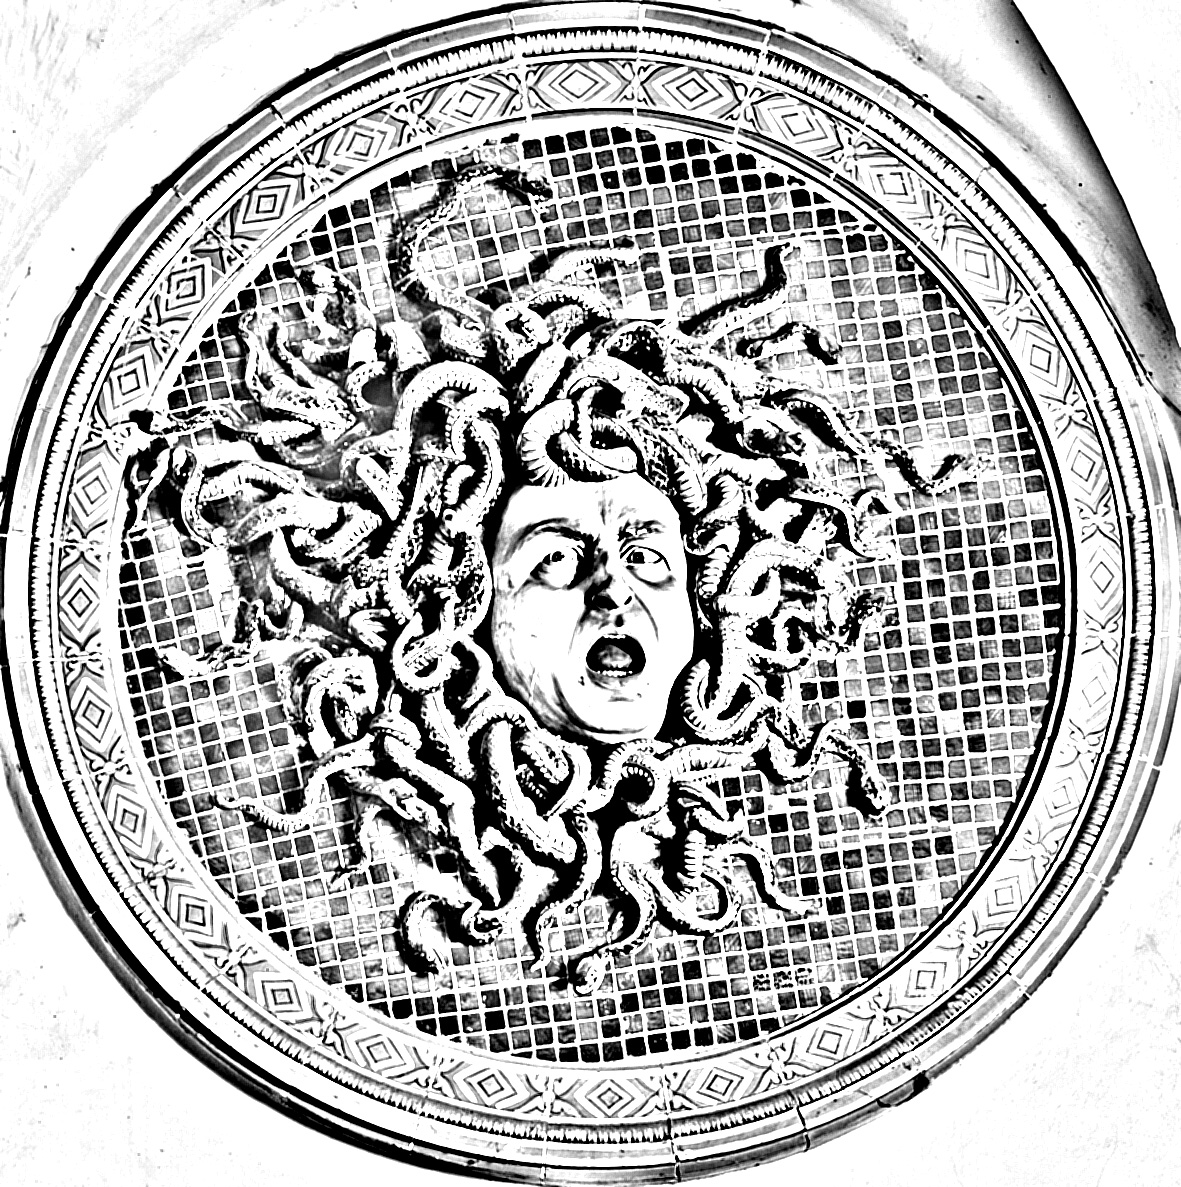
\includegraphics[scale=3.6]{Mengaroni_Ferruccio-Medusa.jpg}
			\end{minipage}
			
			\vspace*{\fill}
			\fboxrule=4pt{
					\fbox
				{
					\begin{minipage}[t][55pt][t]{0.91\linewidth}
					Mengaroni Ferruccio - Medusa - Colorata da: 
					\end{minipage}
				}
				}
			\newpage
			
			%---------- Image ----------
			\thispagestyle{empty}
			\begin{minipage}{0.95\linewidth}
				\centering
				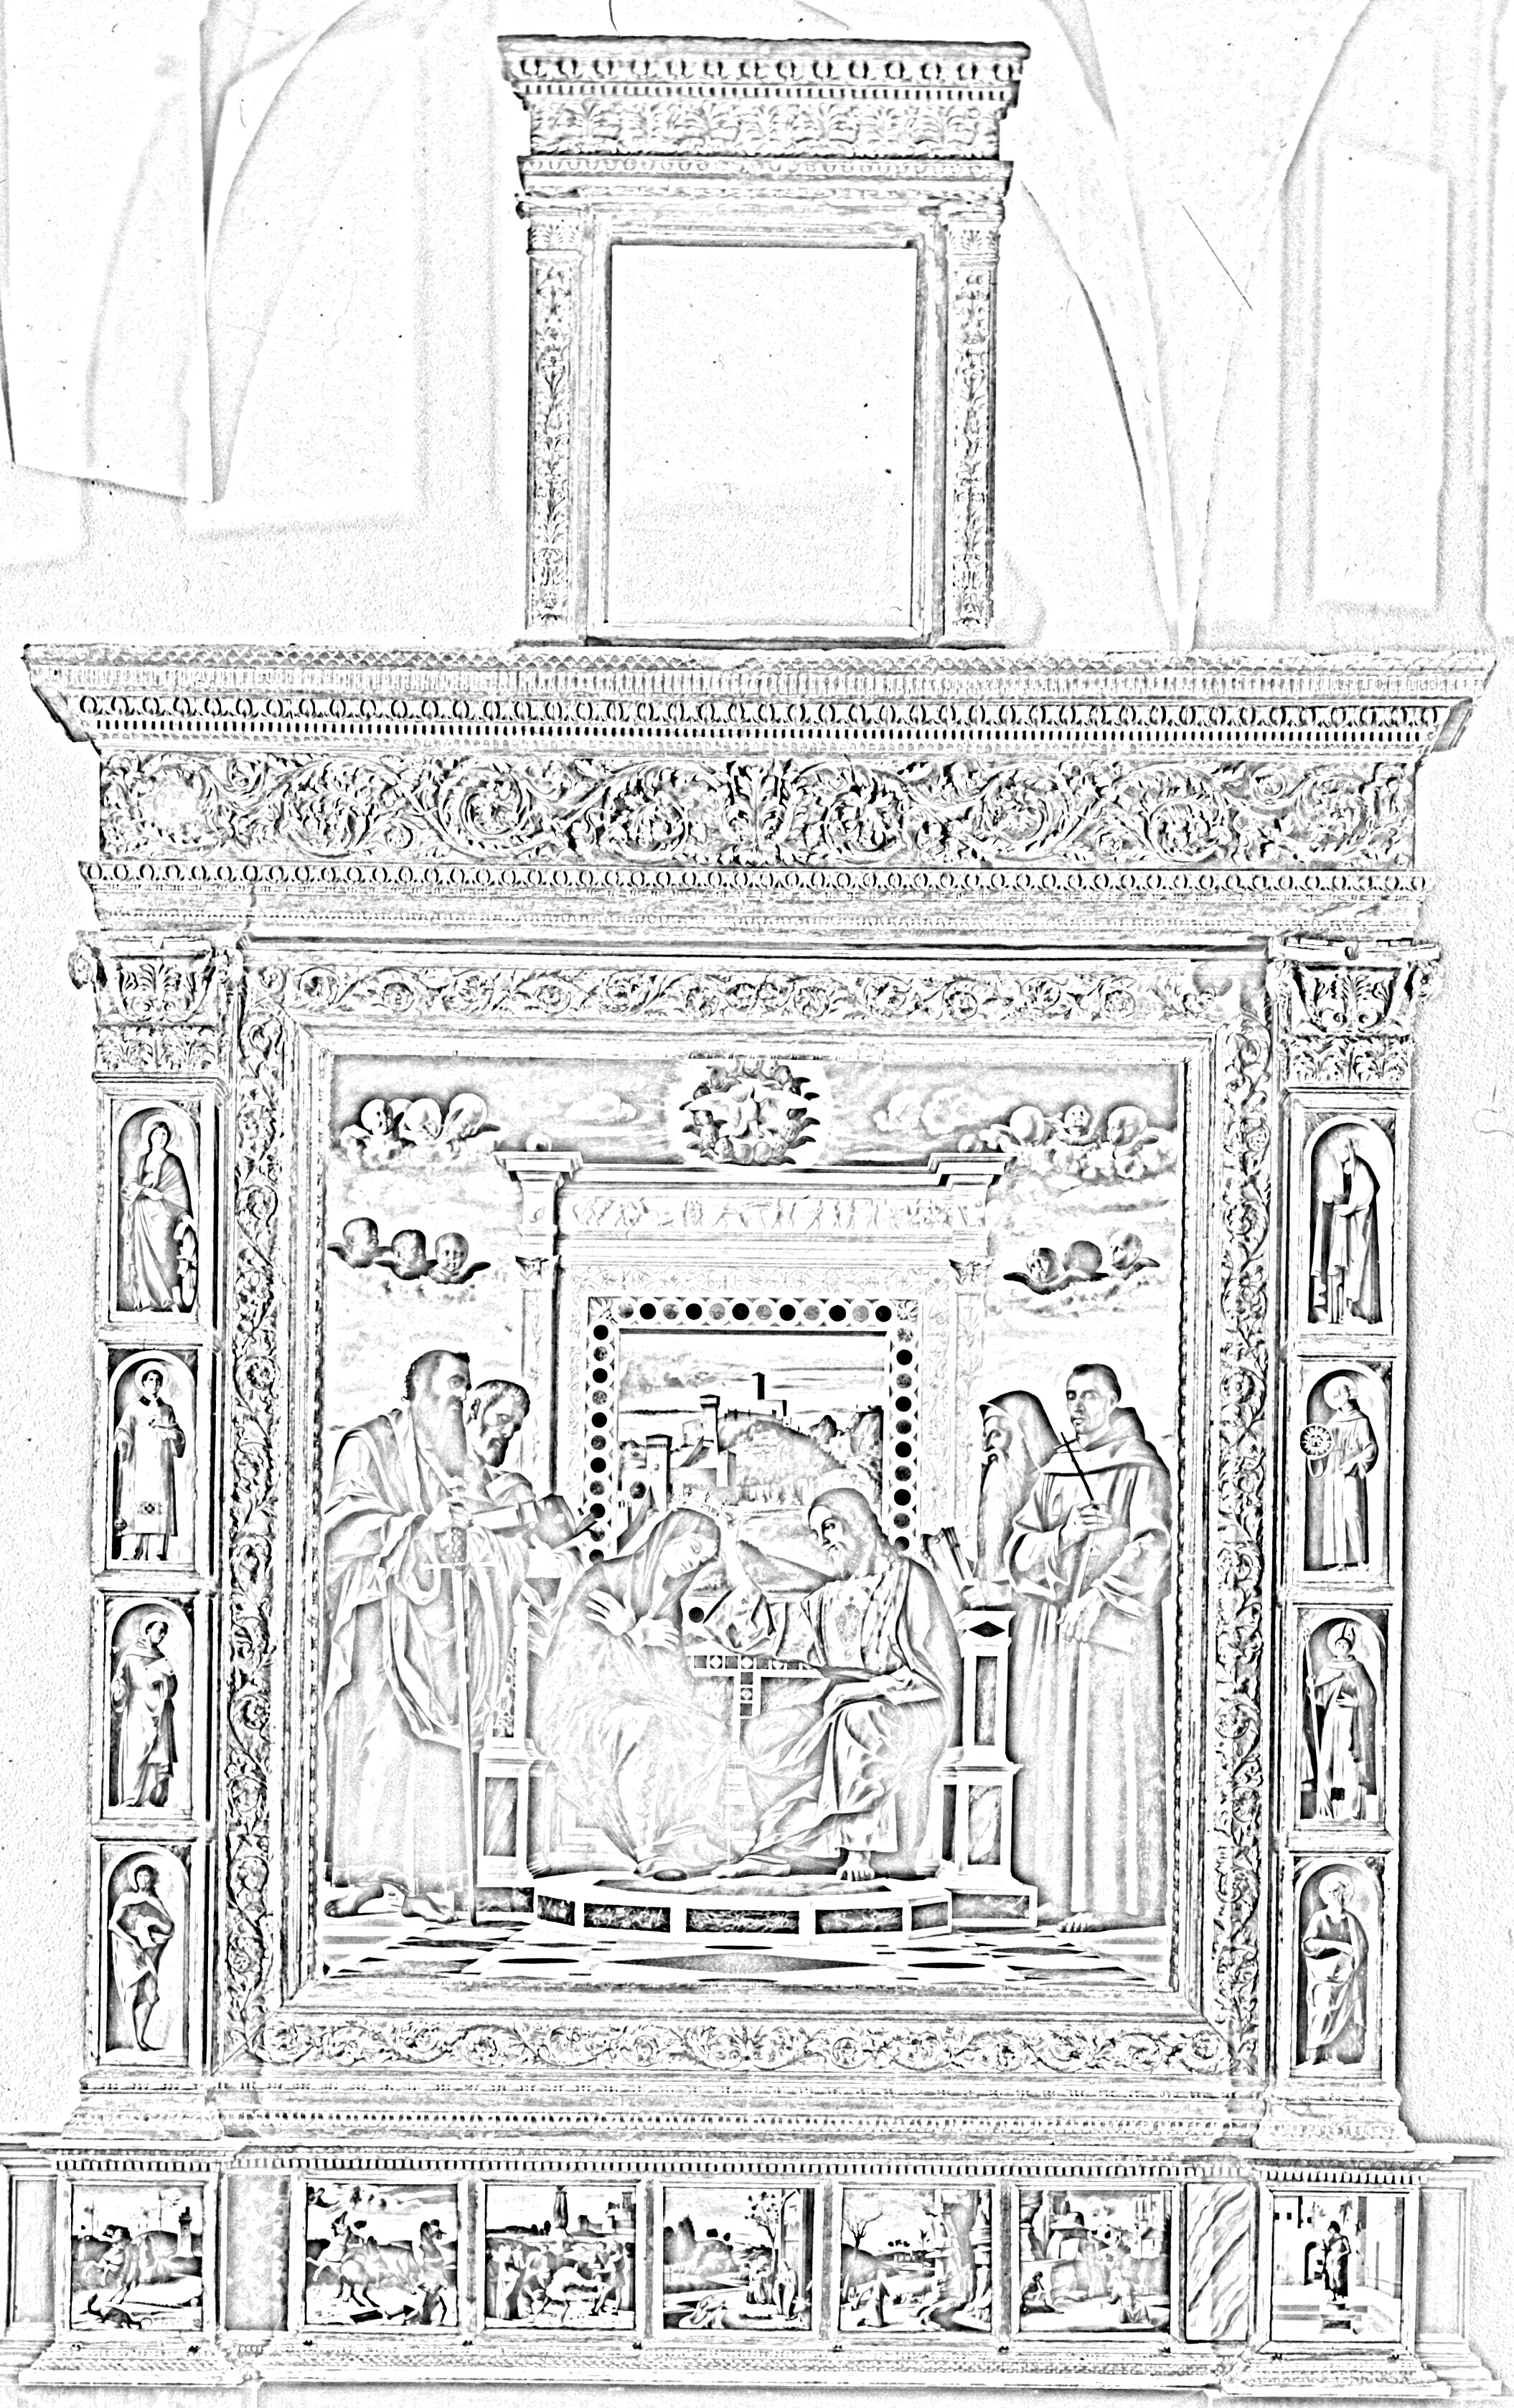
\includegraphics[scale=0.2]{Bellini_Giovanni-Incoronazione_della_Vergine.jpg}
			\end{minipage}
			
			\vspace*{\fill}
			\fboxrule=4pt{
				\fbox
				{
					\begin{minipage}[t][55pt][t]{0.91\linewidth}
						Bellini Giovanni - Incoronazione della Vergine - Colorata da: 
					\end{minipage}
				}
			}
			\newpage
			
			%---------- Image ----------
			\thispagestyle{empty}
			\begin{minipage}{0.95\linewidth}
				\centering
				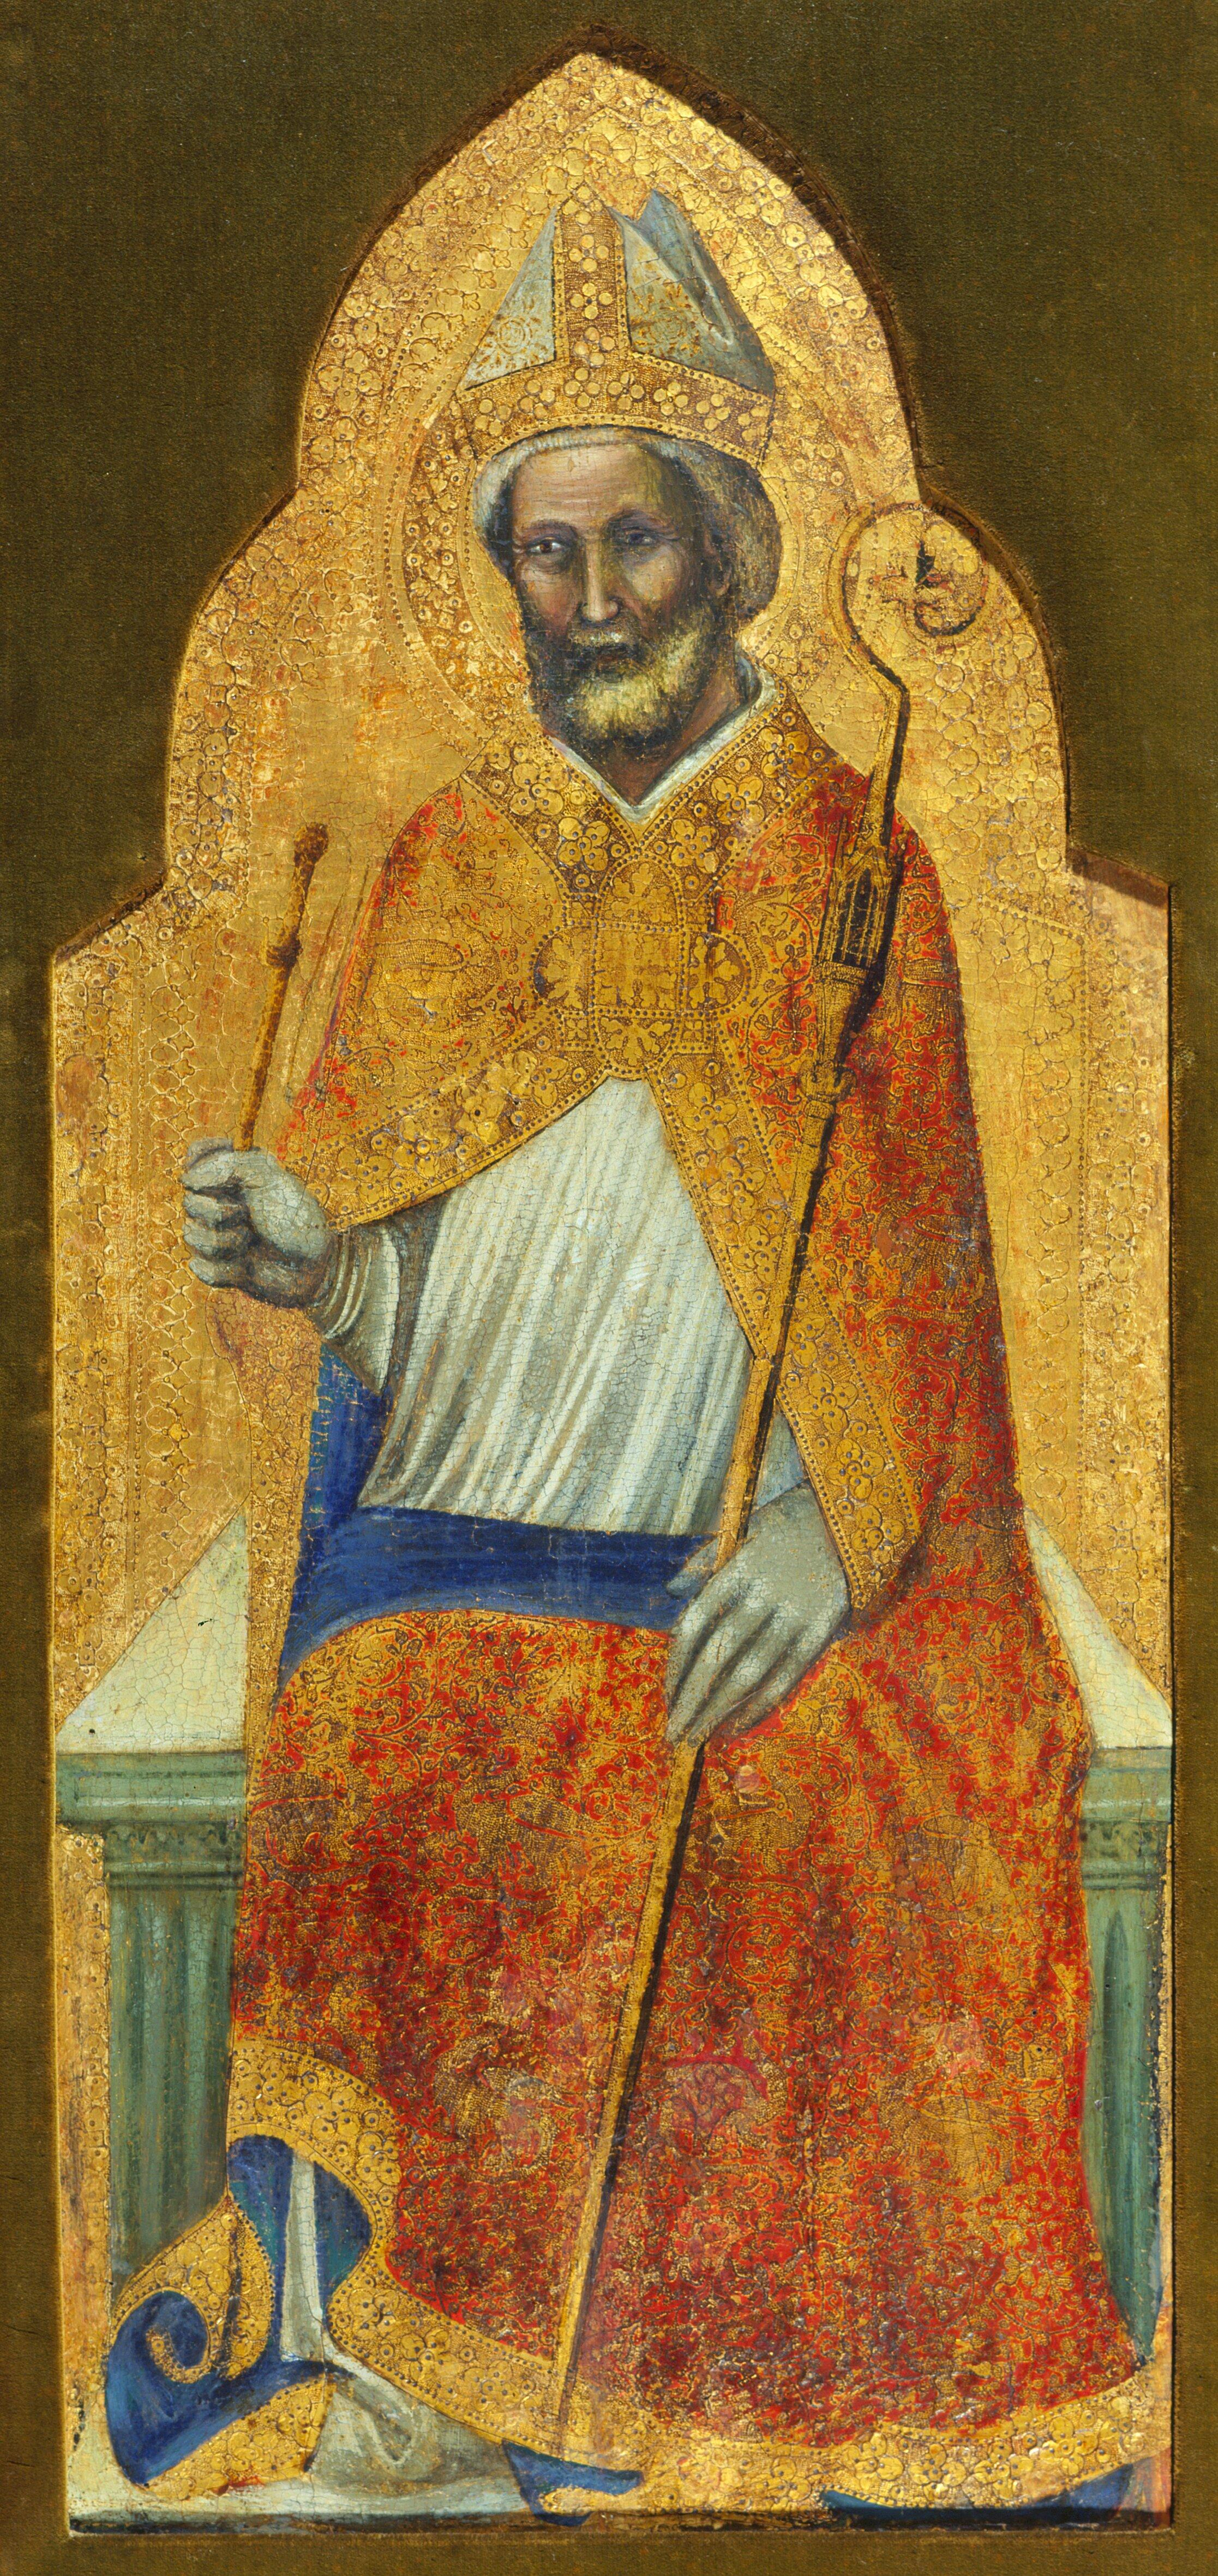
\includegraphics[scale=0.13]{Vitale_da_Bologna-Santo_Ambrogio_in_trono.jpg}
			\end{minipage}
			
			\vspace*{\fill}
			\fboxrule=4pt{
				\fbox
				{
					\begin{minipage}[t][55pt][t]{0.91\linewidth}
						Vitale da Bologna - Sant'Ambrogio in trono - Colorato da: 
					\end{minipage}
				}
			}
			\newpage
			
			%---------- Image ----------
			\thispagestyle{empty}
			\begin{minipage}{0.94\linewidth}
				\centering
				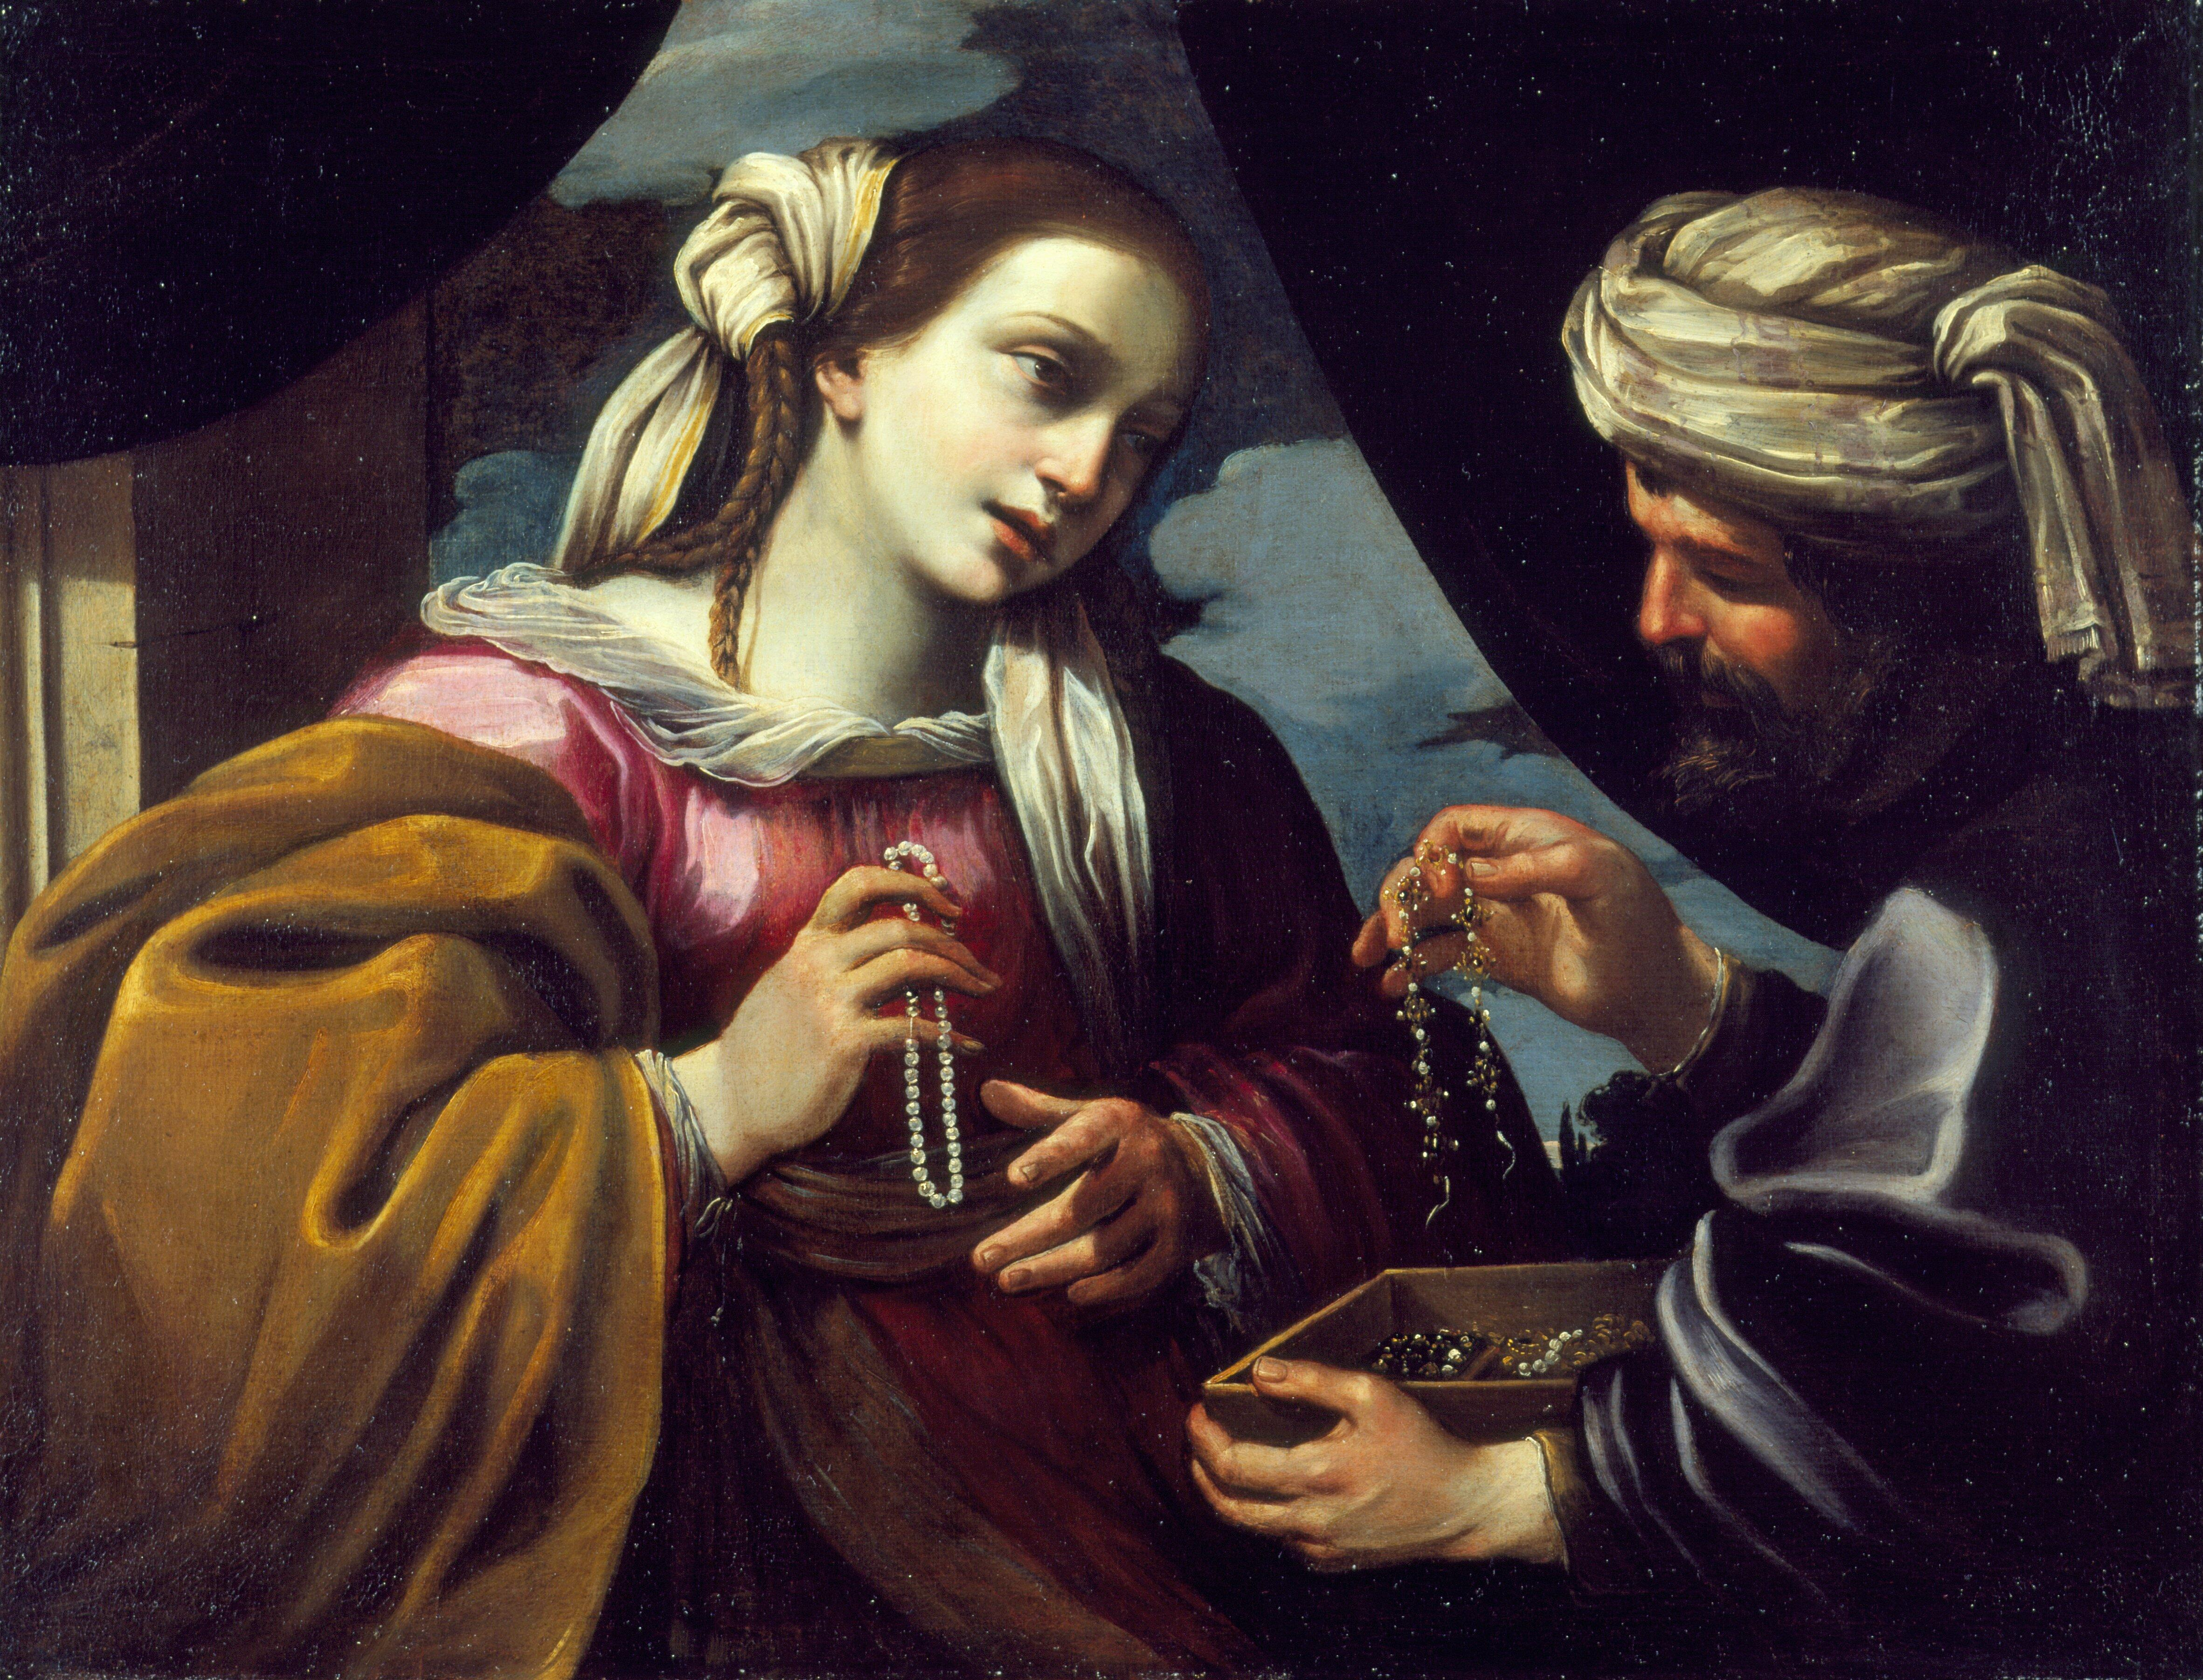
\includegraphics[scale=0.11]{Desani_Pietro-Rebecca_ed_Eleazar.jpg}
			\end{minipage}
			
			\vspace*{\fill}
			\fboxrule=4pt{
				\fbox
				{
					\begin{minipage}[t][55pt][t]{0.91\linewidth}
						Desani Pietro - Rebecca ed Eleazar - Colorato da: 
					\end{minipage}
				}
			}
			\newpage
			
			%---------- Image ----------
			\thispagestyle{empty}
			\begin{minipage}{0.79\linewidth}
				\centering
				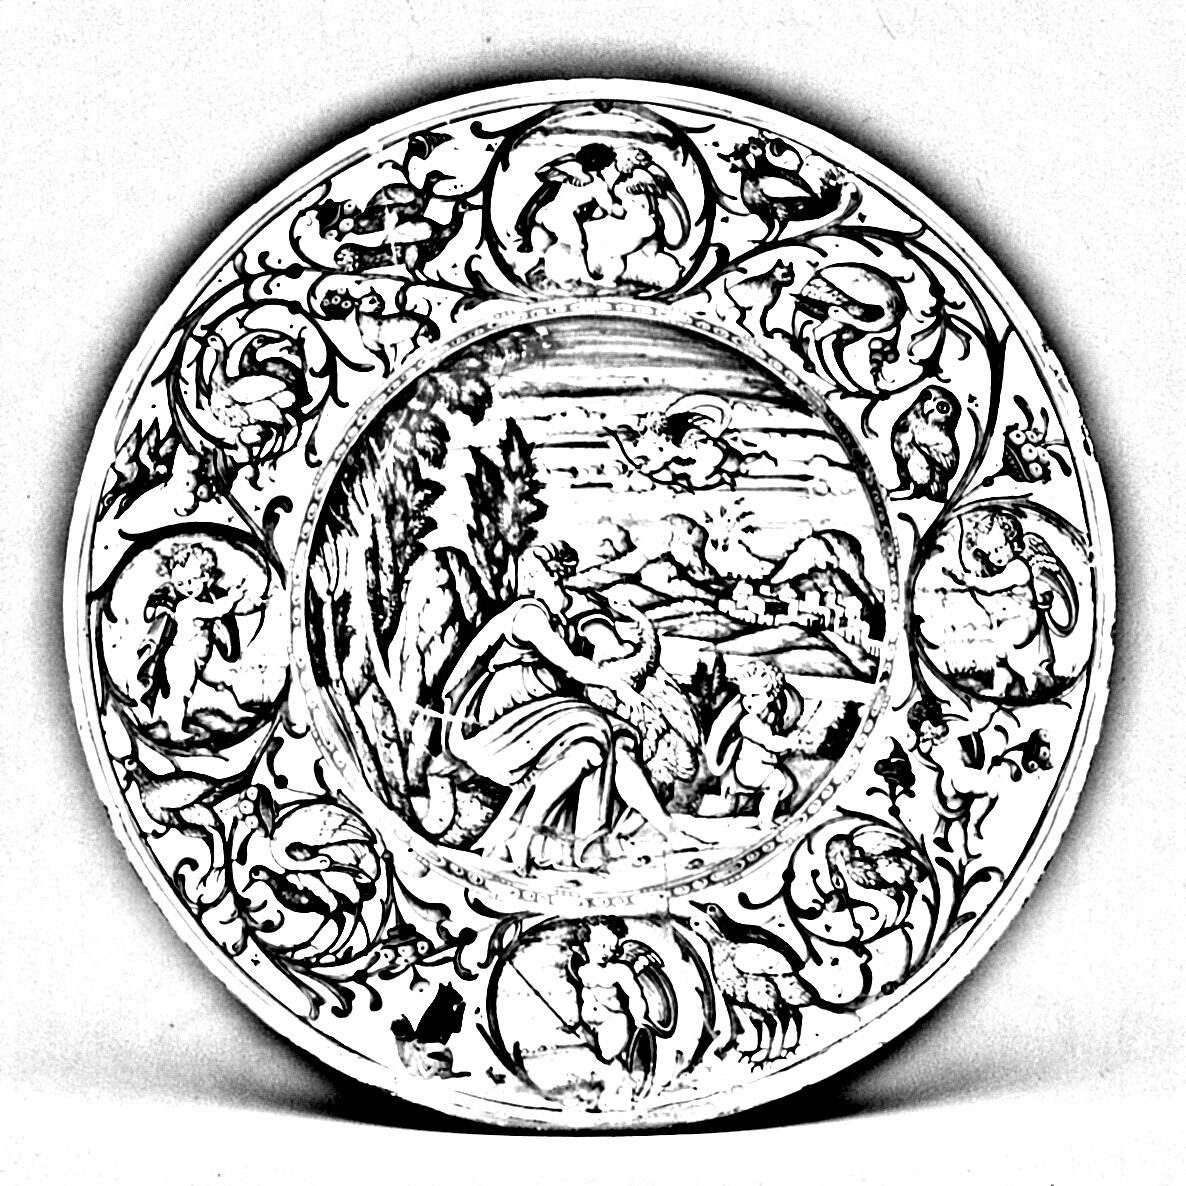
\includegraphics[scale=3.7]{Giovanni_Antonio_Garella-Leda_e_il_cigno.jpg}
			\end{minipage}
			
			\vspace*{\fill}
			\fboxrule=4pt{
				\fbox
				{
					\begin{minipage}[t][55pt][t]{0.91\linewidth}
						 Giovanni Antonio Garella - Leda e il Cigno - Colorato da: 
					\end{minipage}
				}
			}
			\newpage
			
			%---------- Image ----------
			\thispagestyle{empty}
			\begin{minipage}{0.94\linewidth}
				\centering
				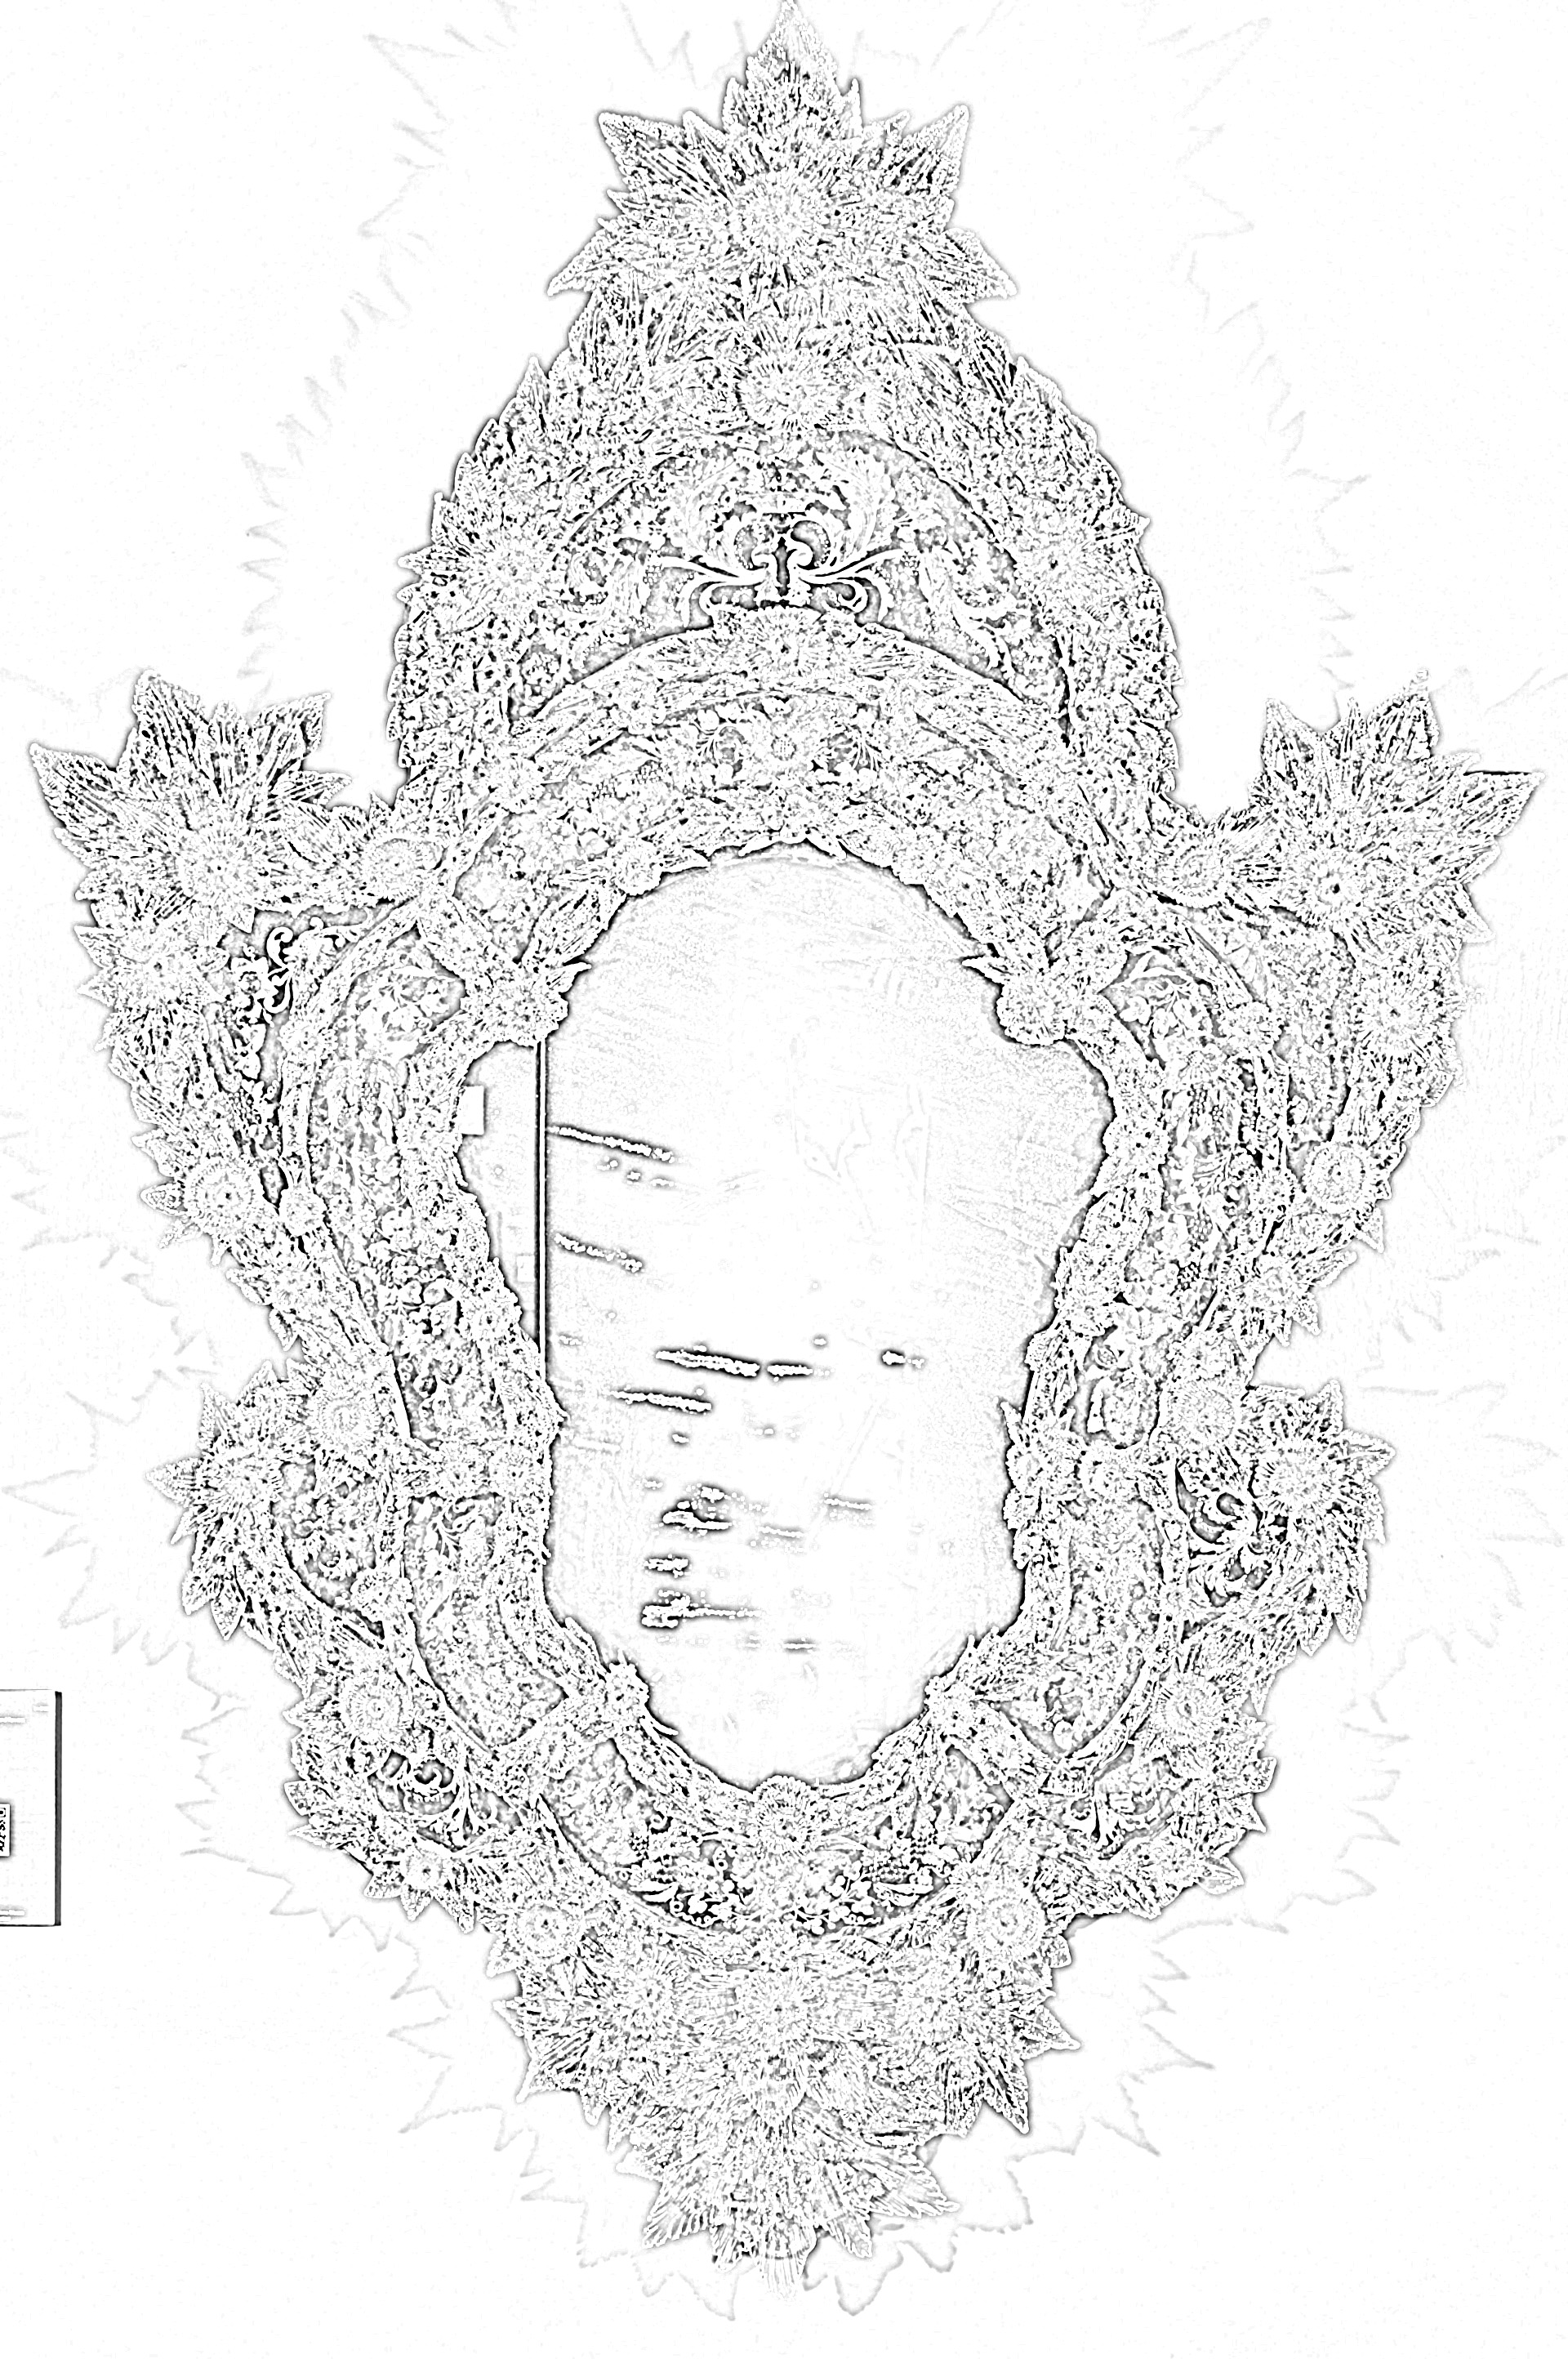
\includegraphics[scale=0.8]{Specchio_di_Murano.jpg}
			\end{minipage}
			
			\vspace*{\fill}
			\fboxrule=4pt{
				\fbox
				{
					\begin{minipage}[t][55pt][t]{0.91\linewidth}
						Specchio in vetro di Murano - Colorato da: 
					\end{minipage}
				}
			}
			\newpage
			
			%---------- Image ----------
			\thispagestyle{empty}
			\begin{minipage}{0.95\linewidth}
				\centering
				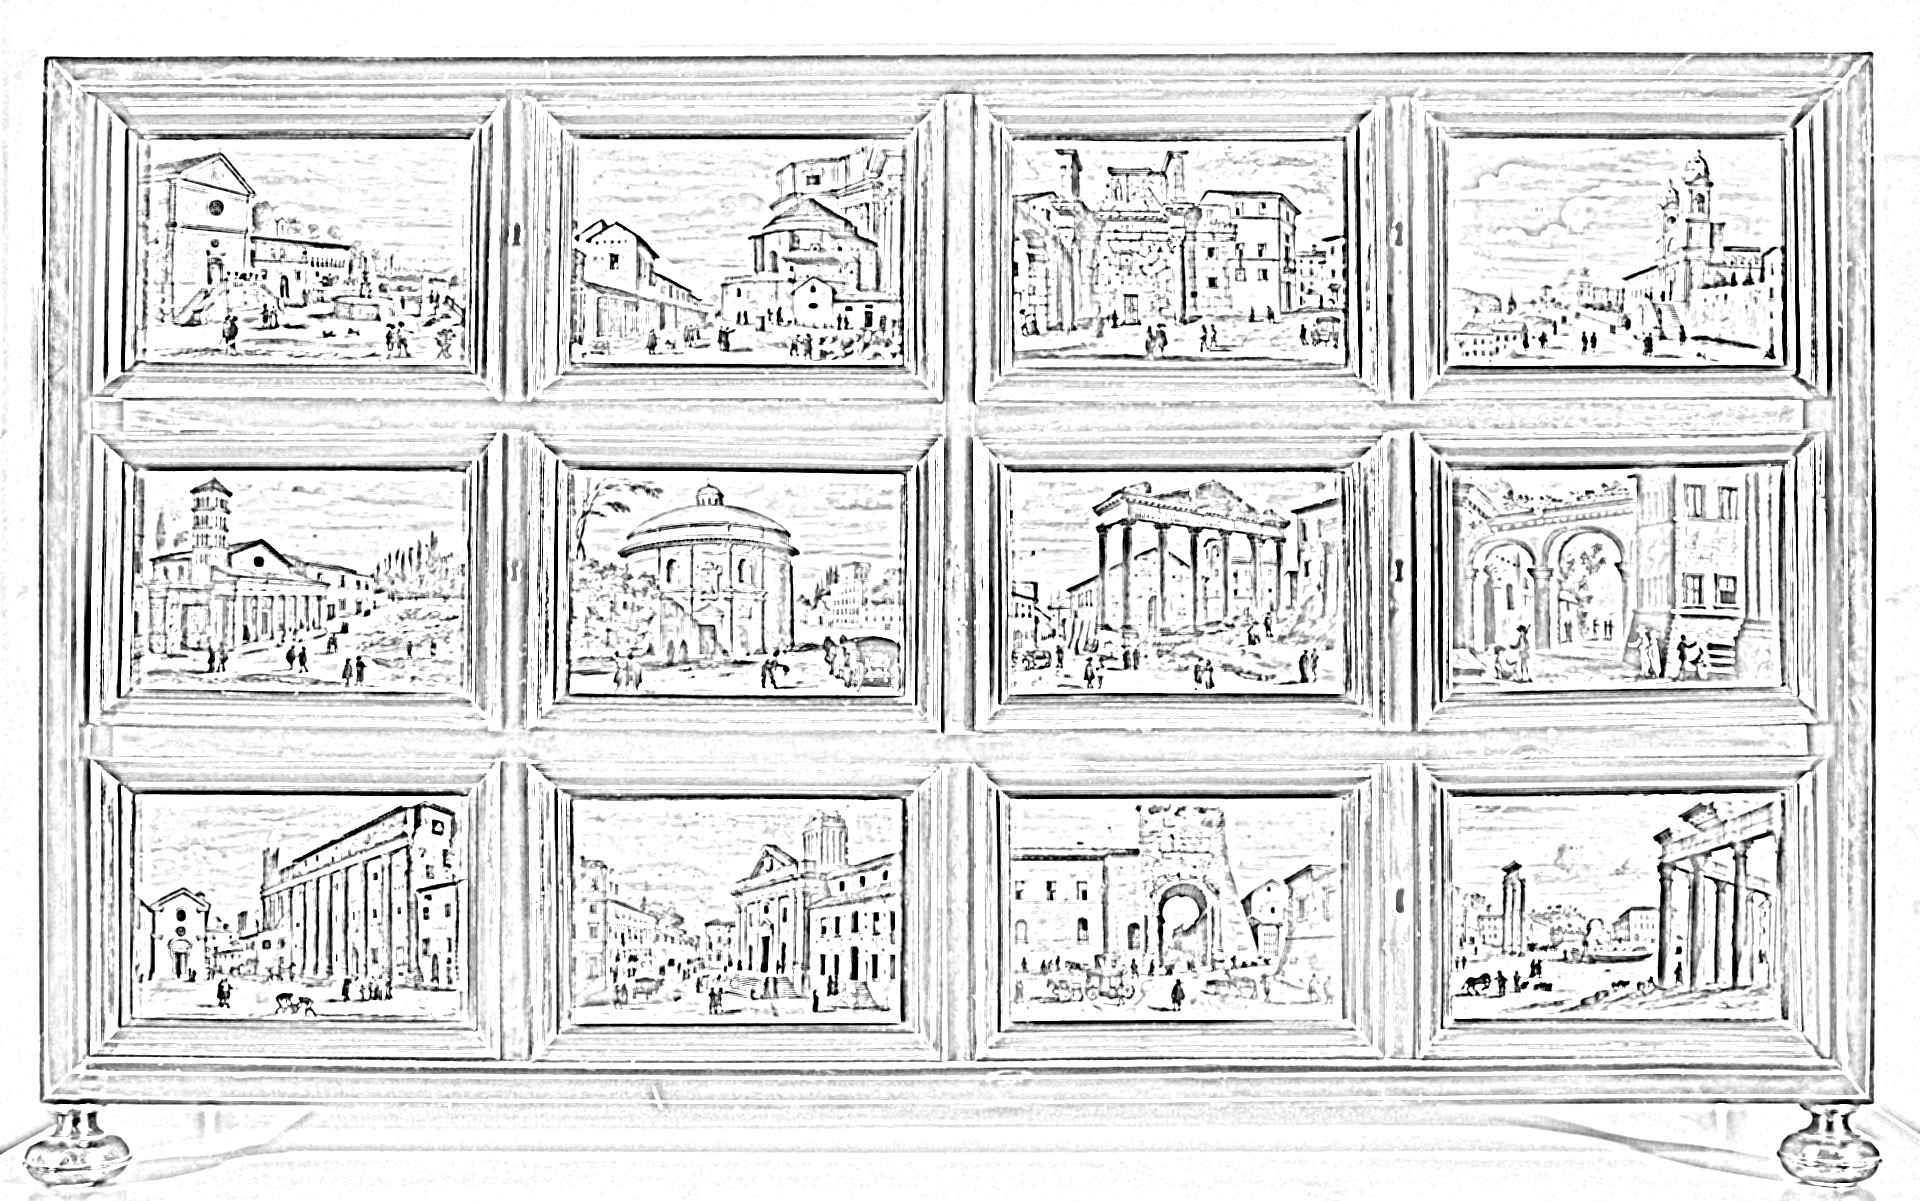
\includegraphics[scale=0.9]{Vedute_di_Roma_1.jpg}
			\end{minipage}
			
			\vspace*{\fill}
			\fboxrule=4pt{
				\fbox
				{
					\begin{minipage}[t][55pt][t]{0.91\linewidth}
						Stipo con vedute di Roma - Colorate da: 
					\end{minipage}
				}
			}
			\newpage
			
			%---------- Image ----------
			\thispagestyle{empty}
			\begin{minipage}{0.94\linewidth}
				\centering
				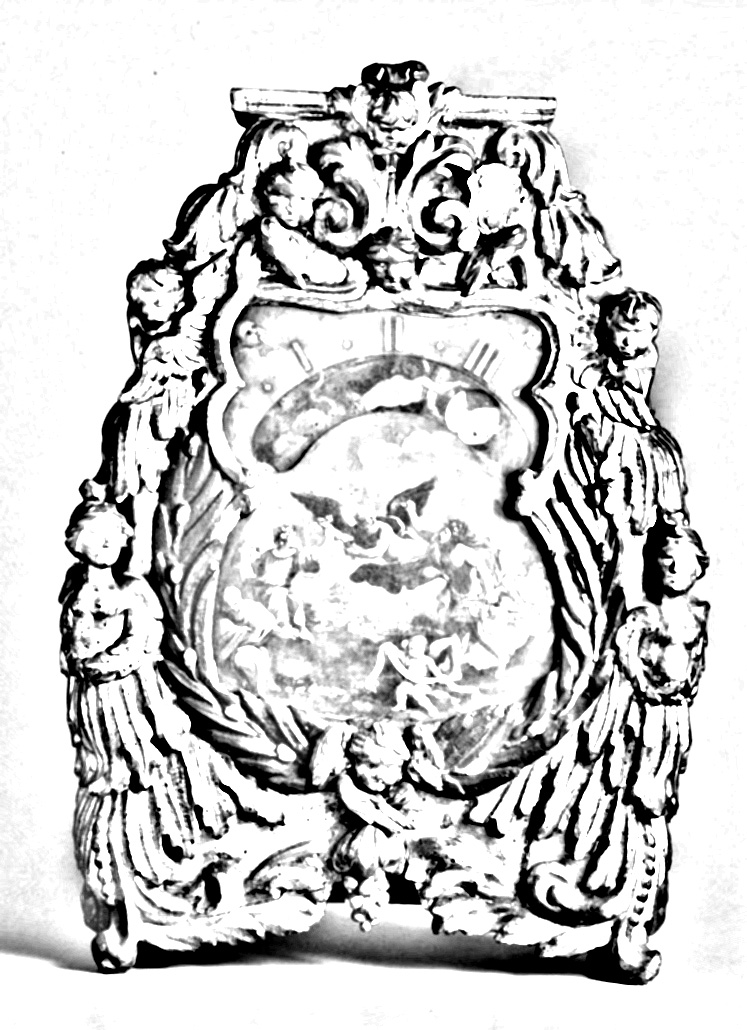
\includegraphics[scale=0.6]{Orologio_notturno.jpg}
			\end{minipage}
			
			\vspace*{\fill}
			\fboxrule=4pt{
				\fbox
				{
					\begin{minipage}[t][55pt][t]{0.91\linewidth}
						Orologio notturno - Colorato da: 
					\end{minipage}
				}
			}
			\newpage
			
			%---------- Image ----------
			\thispagestyle{empty}
			\begin{minipage}{0.94\linewidth}
				\centering
				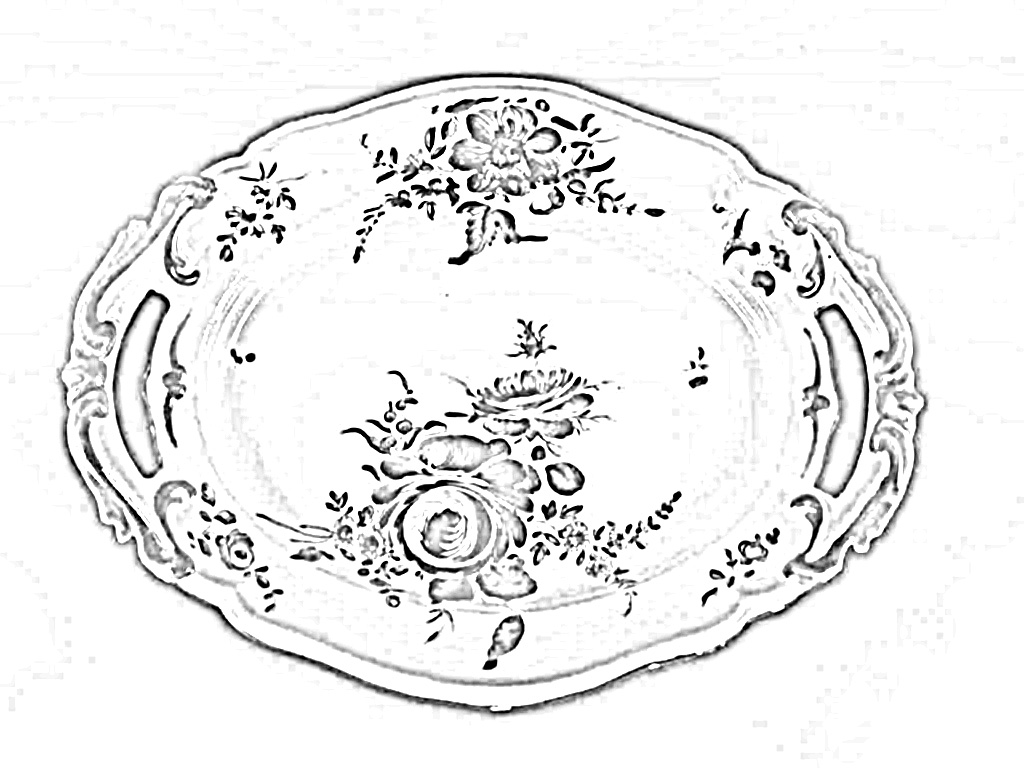
\includegraphics[scale=2]{Scacciani_Antonio-Vassoio-Rosa.jpg}
			\end{minipage}
			
			\vspace*{\fill}
			\fboxrule=4pt{
				\fbox
				{
					\begin{minipage}[t][55pt][t]{0.91\linewidth}
						Scacciani Antonio - Vassoio - Rosa - Colorato da: 
					\end{minipage}
				}
			}
			\newpage
			
			%---------- Image ----------
			\thispagestyle{empty}
			\begin{minipage}{0.93\linewidth}
				\centering
				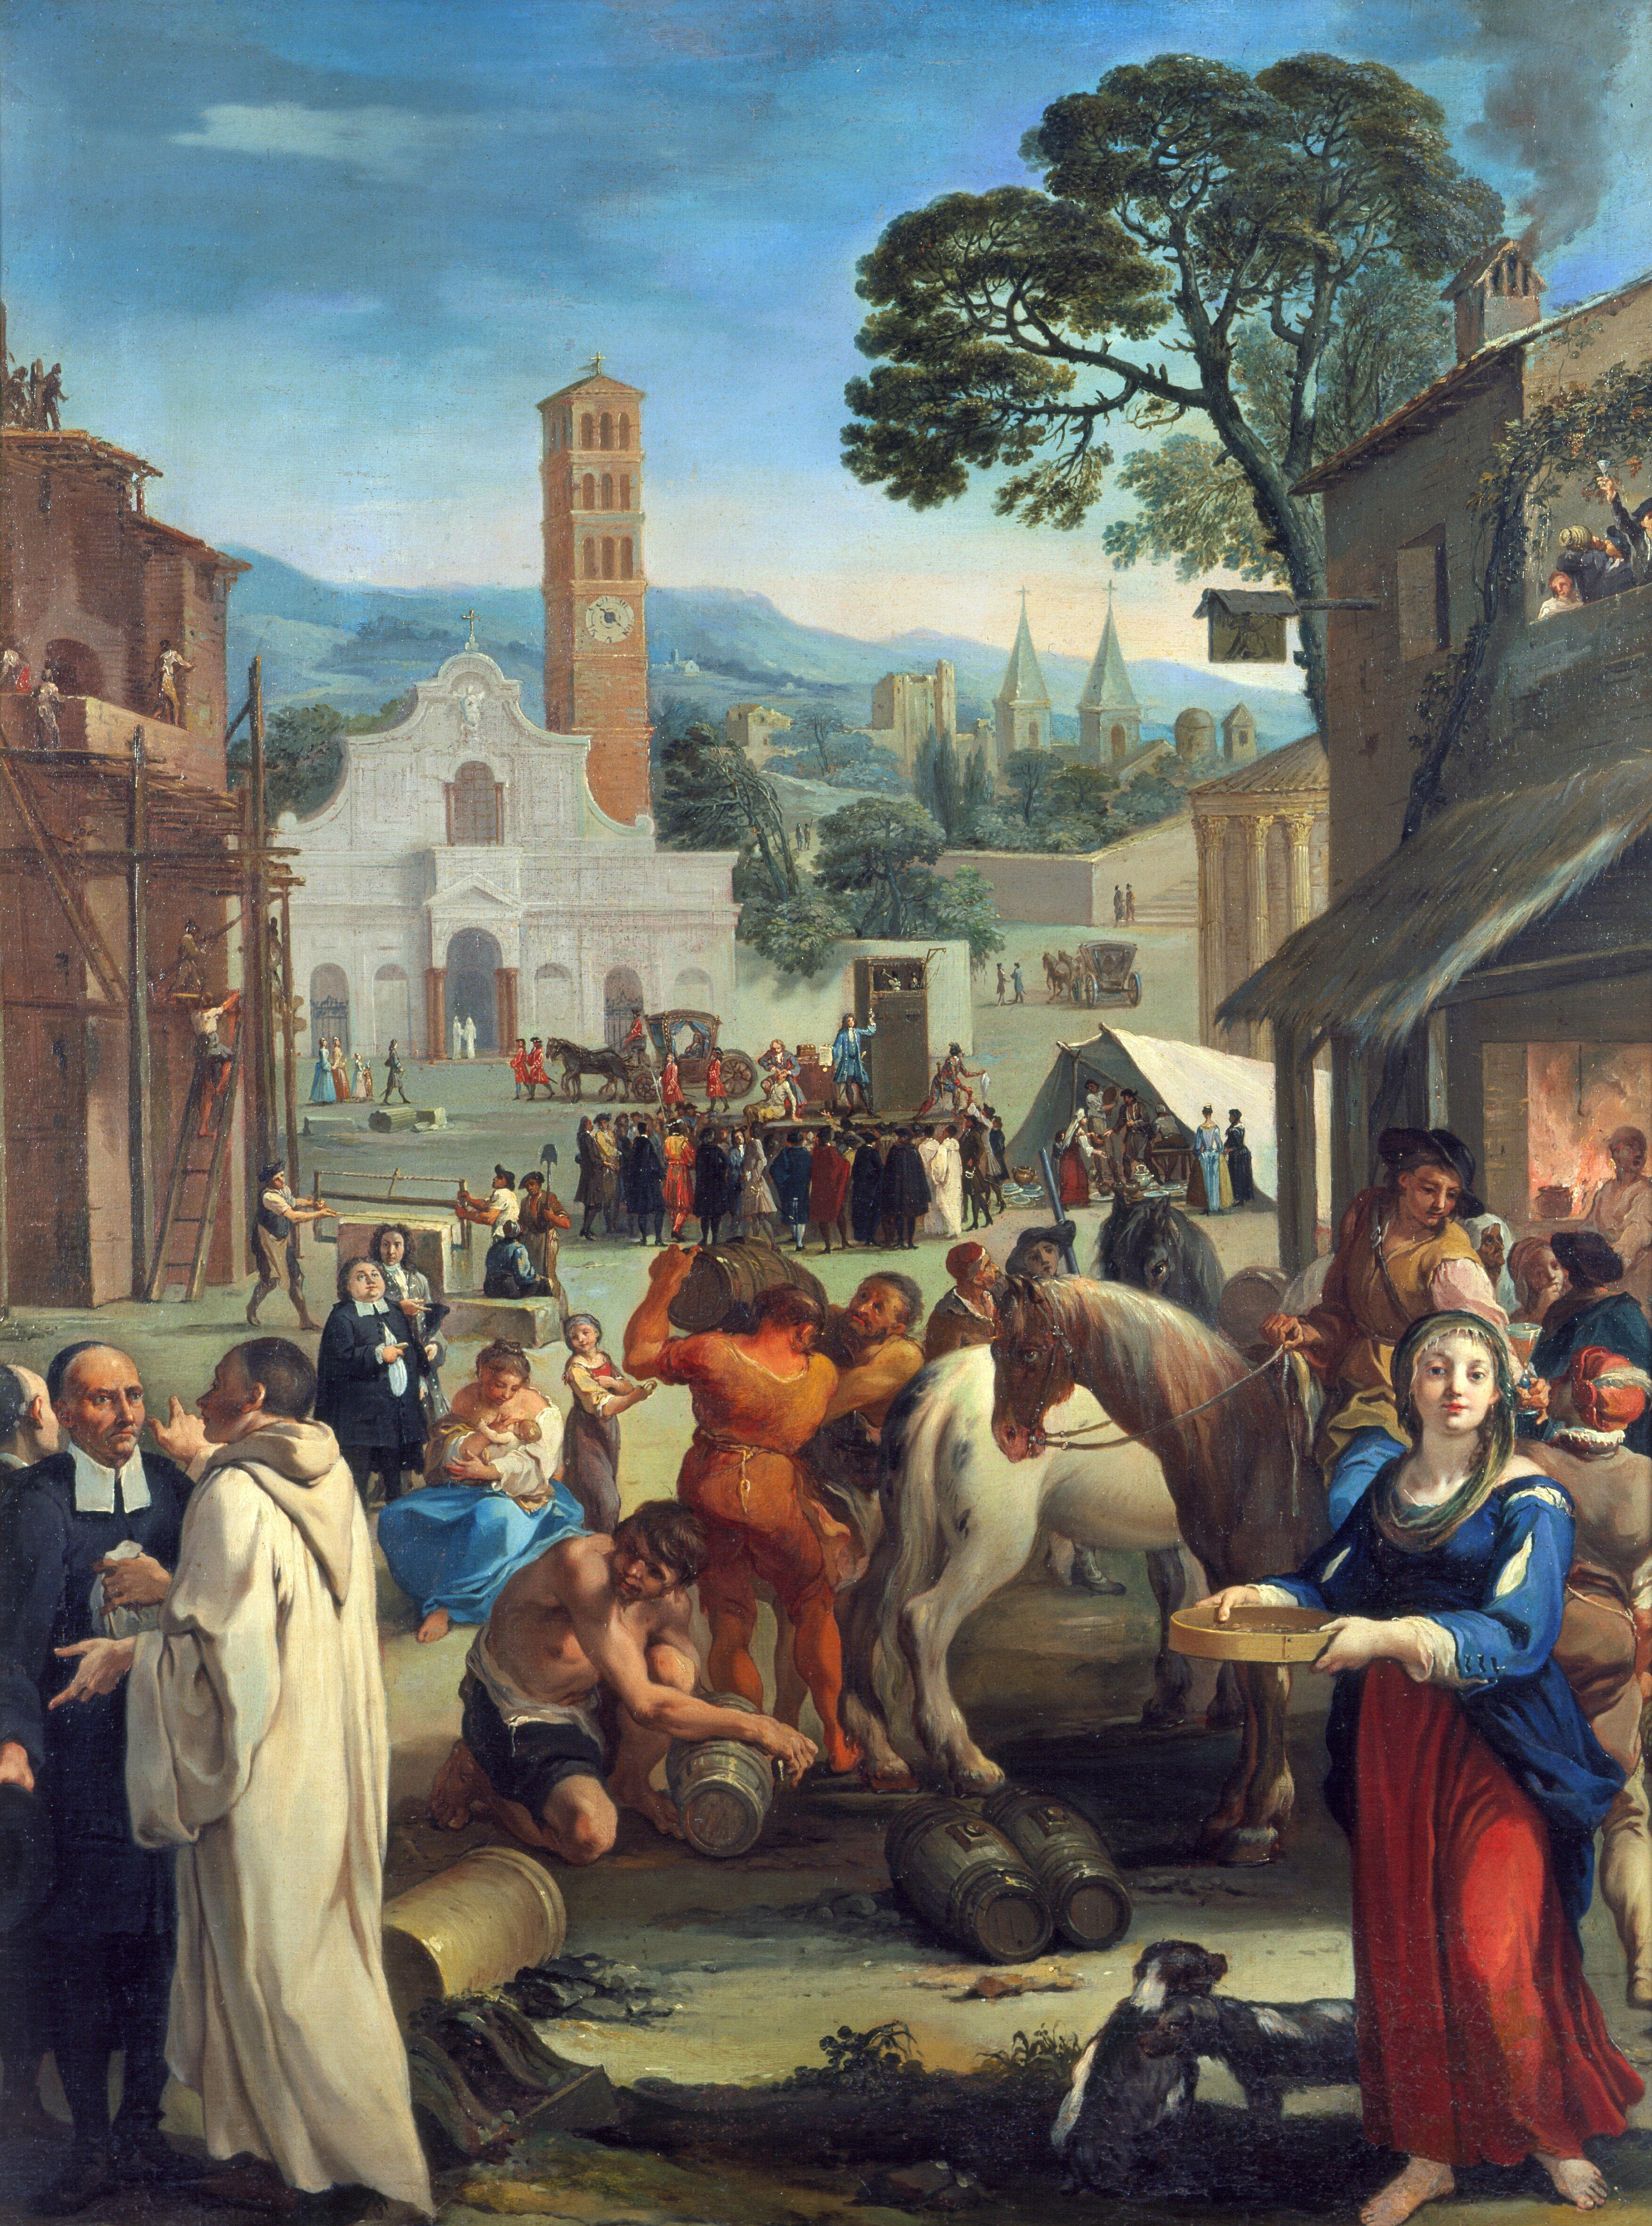
\includegraphics[scale=0.13]{Milani_Aureliano-Mercato.jpg}
			\end{minipage}
			
			\vspace*{\fill}
			\fboxrule=4pt{
				\fbox
				{
					\begin{minipage}[t][55pt][t]{0.91\linewidth}
						Milani Aureliano - Mercato - Colorato da: 
					\end{minipage}
				}
			}
			\newpage
			
			%---------- Image ----------
			\thispagestyle{empty}
			\begin{minipage}{0.93\linewidth}
				\centering
				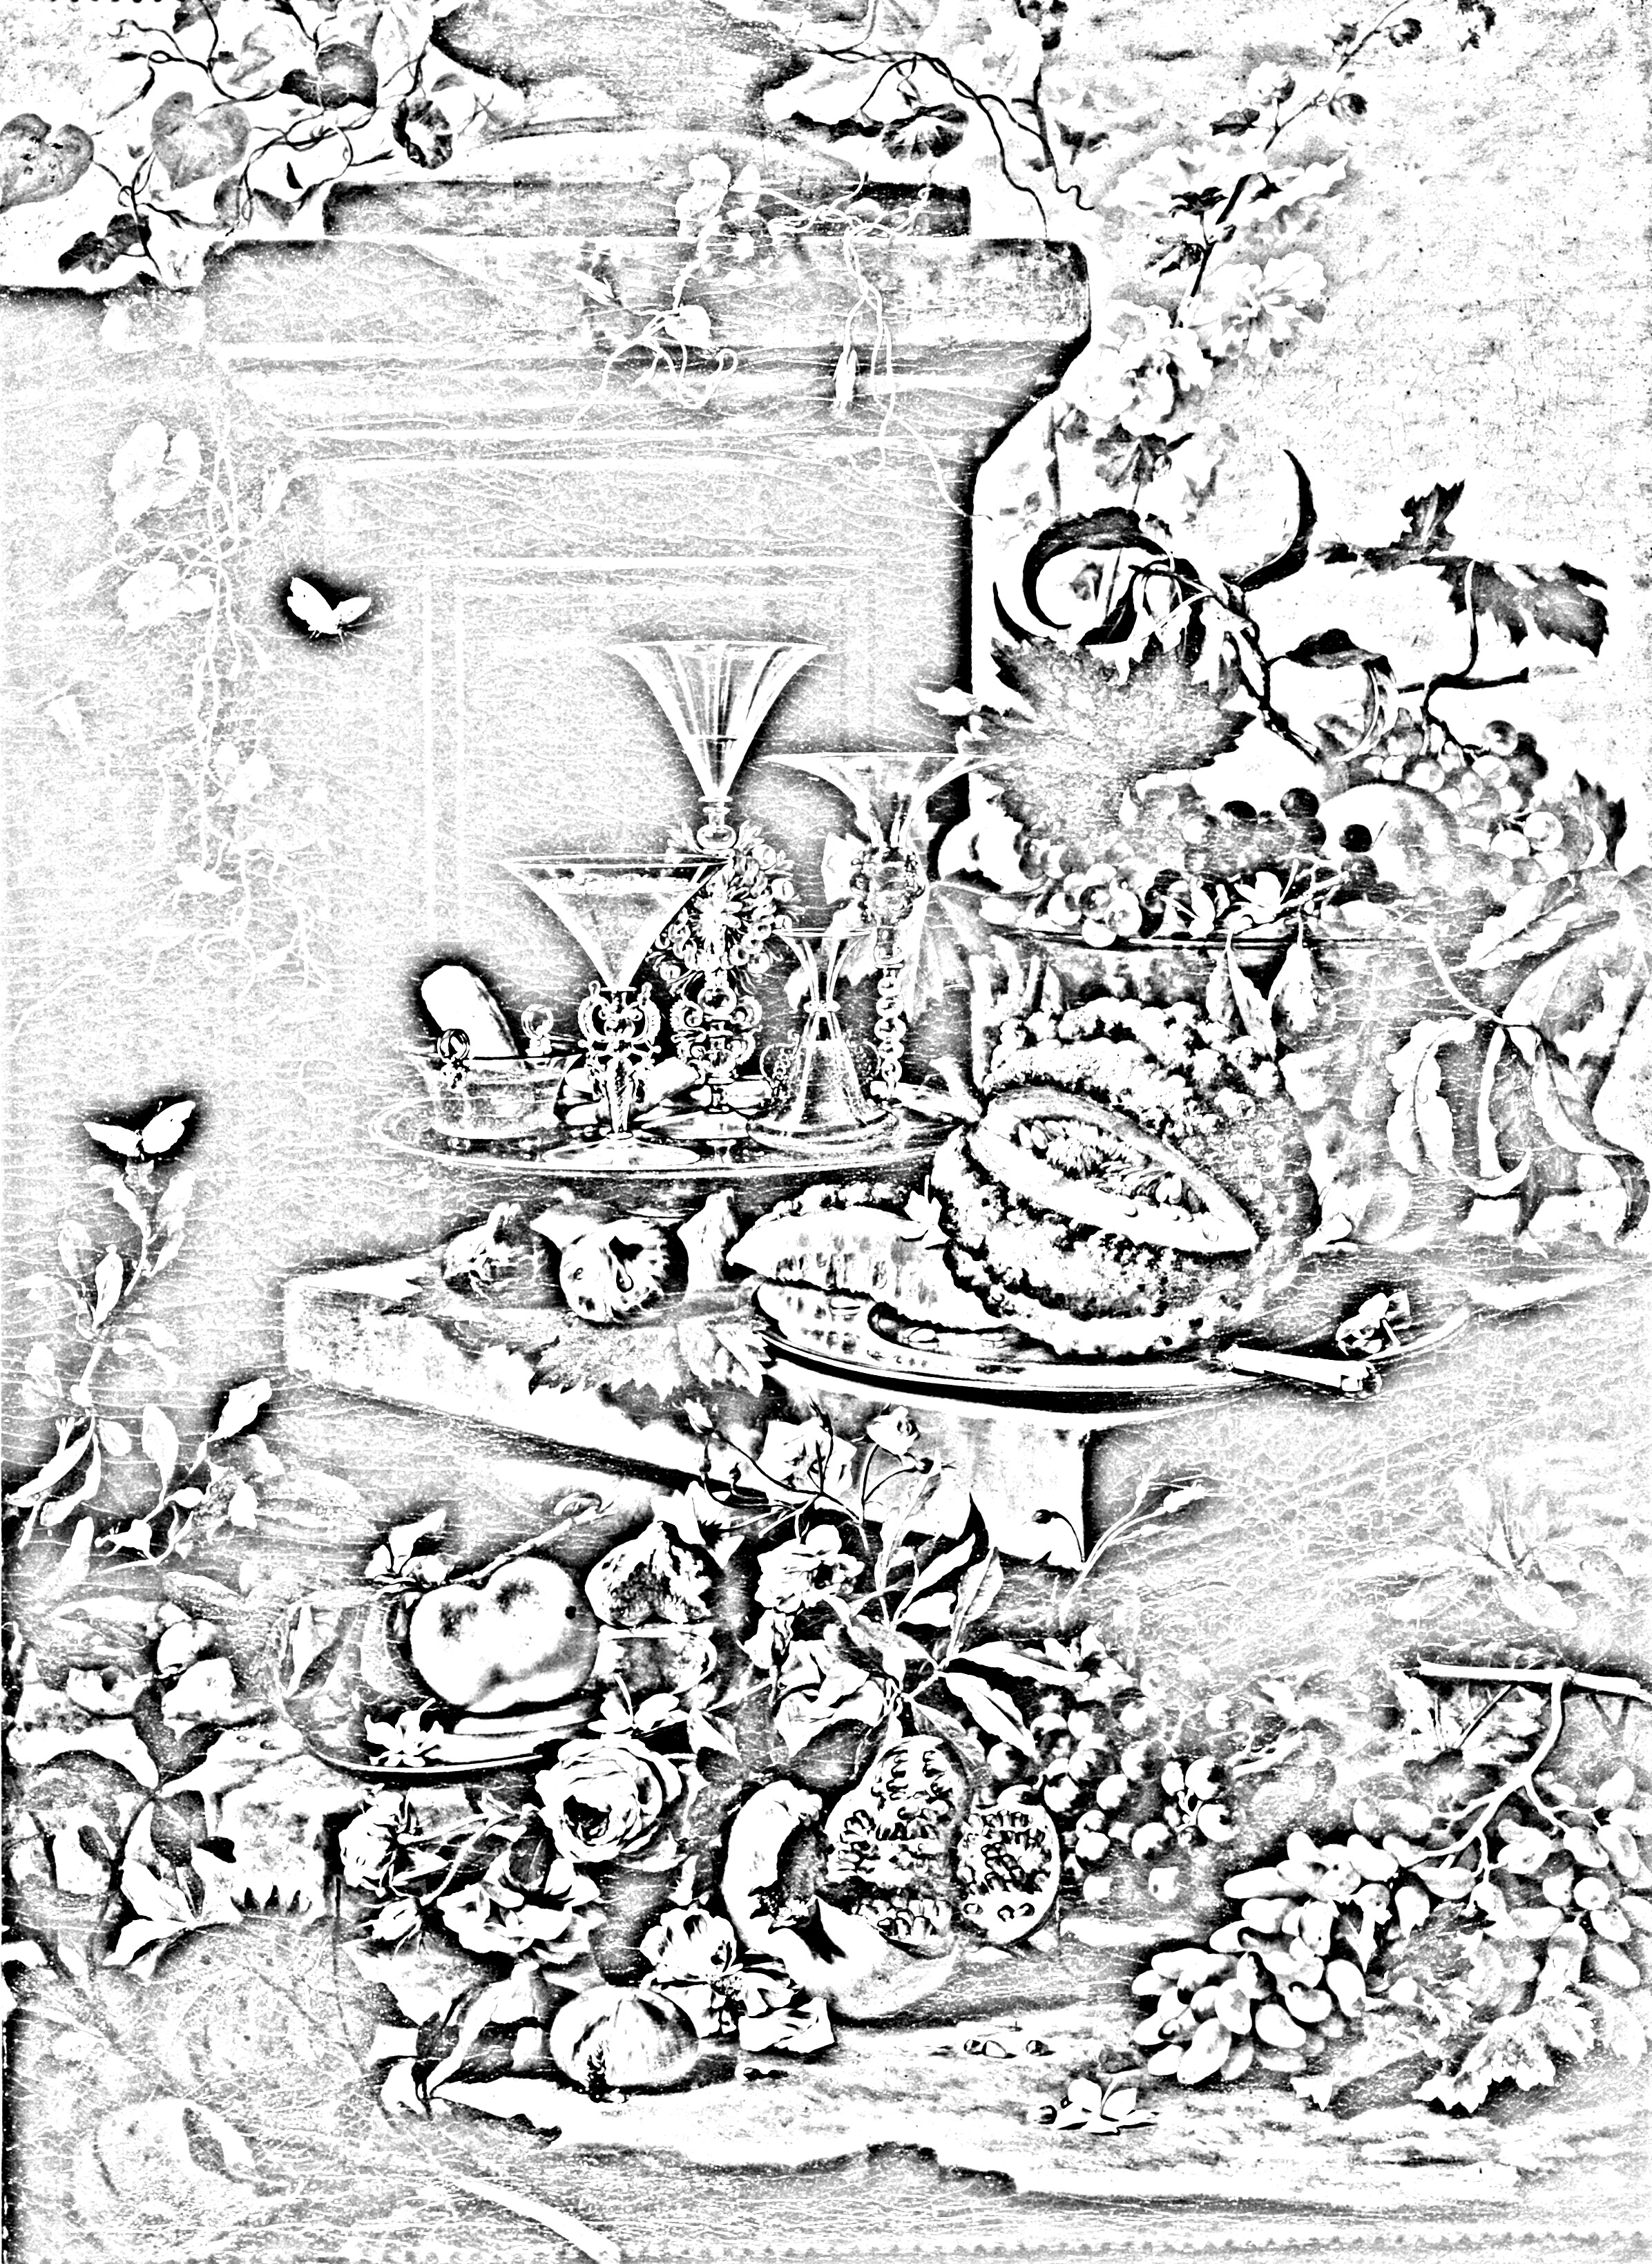
\includegraphics[scale=0.2]{Berentz_Christian-Fiori_e_frutta_con_bicchieri_di_cristallo.jpg}
			\end{minipage}
			
			\vspace*{\fill}
			\fboxrule=4pt{
				\fbox
				{
					\begin{minipage}[t][55pt][t]{0.91\linewidth}
						Berentz Christian - Fiori e frutta con bicchieri di cristallo - Colorati da: 
					\end{minipage}
				}
			}
			\newpage
			
			%---------- Image ----------
			\thispagestyle{empty}
			\begin{minipage}{0.93\linewidth}
				\centering
				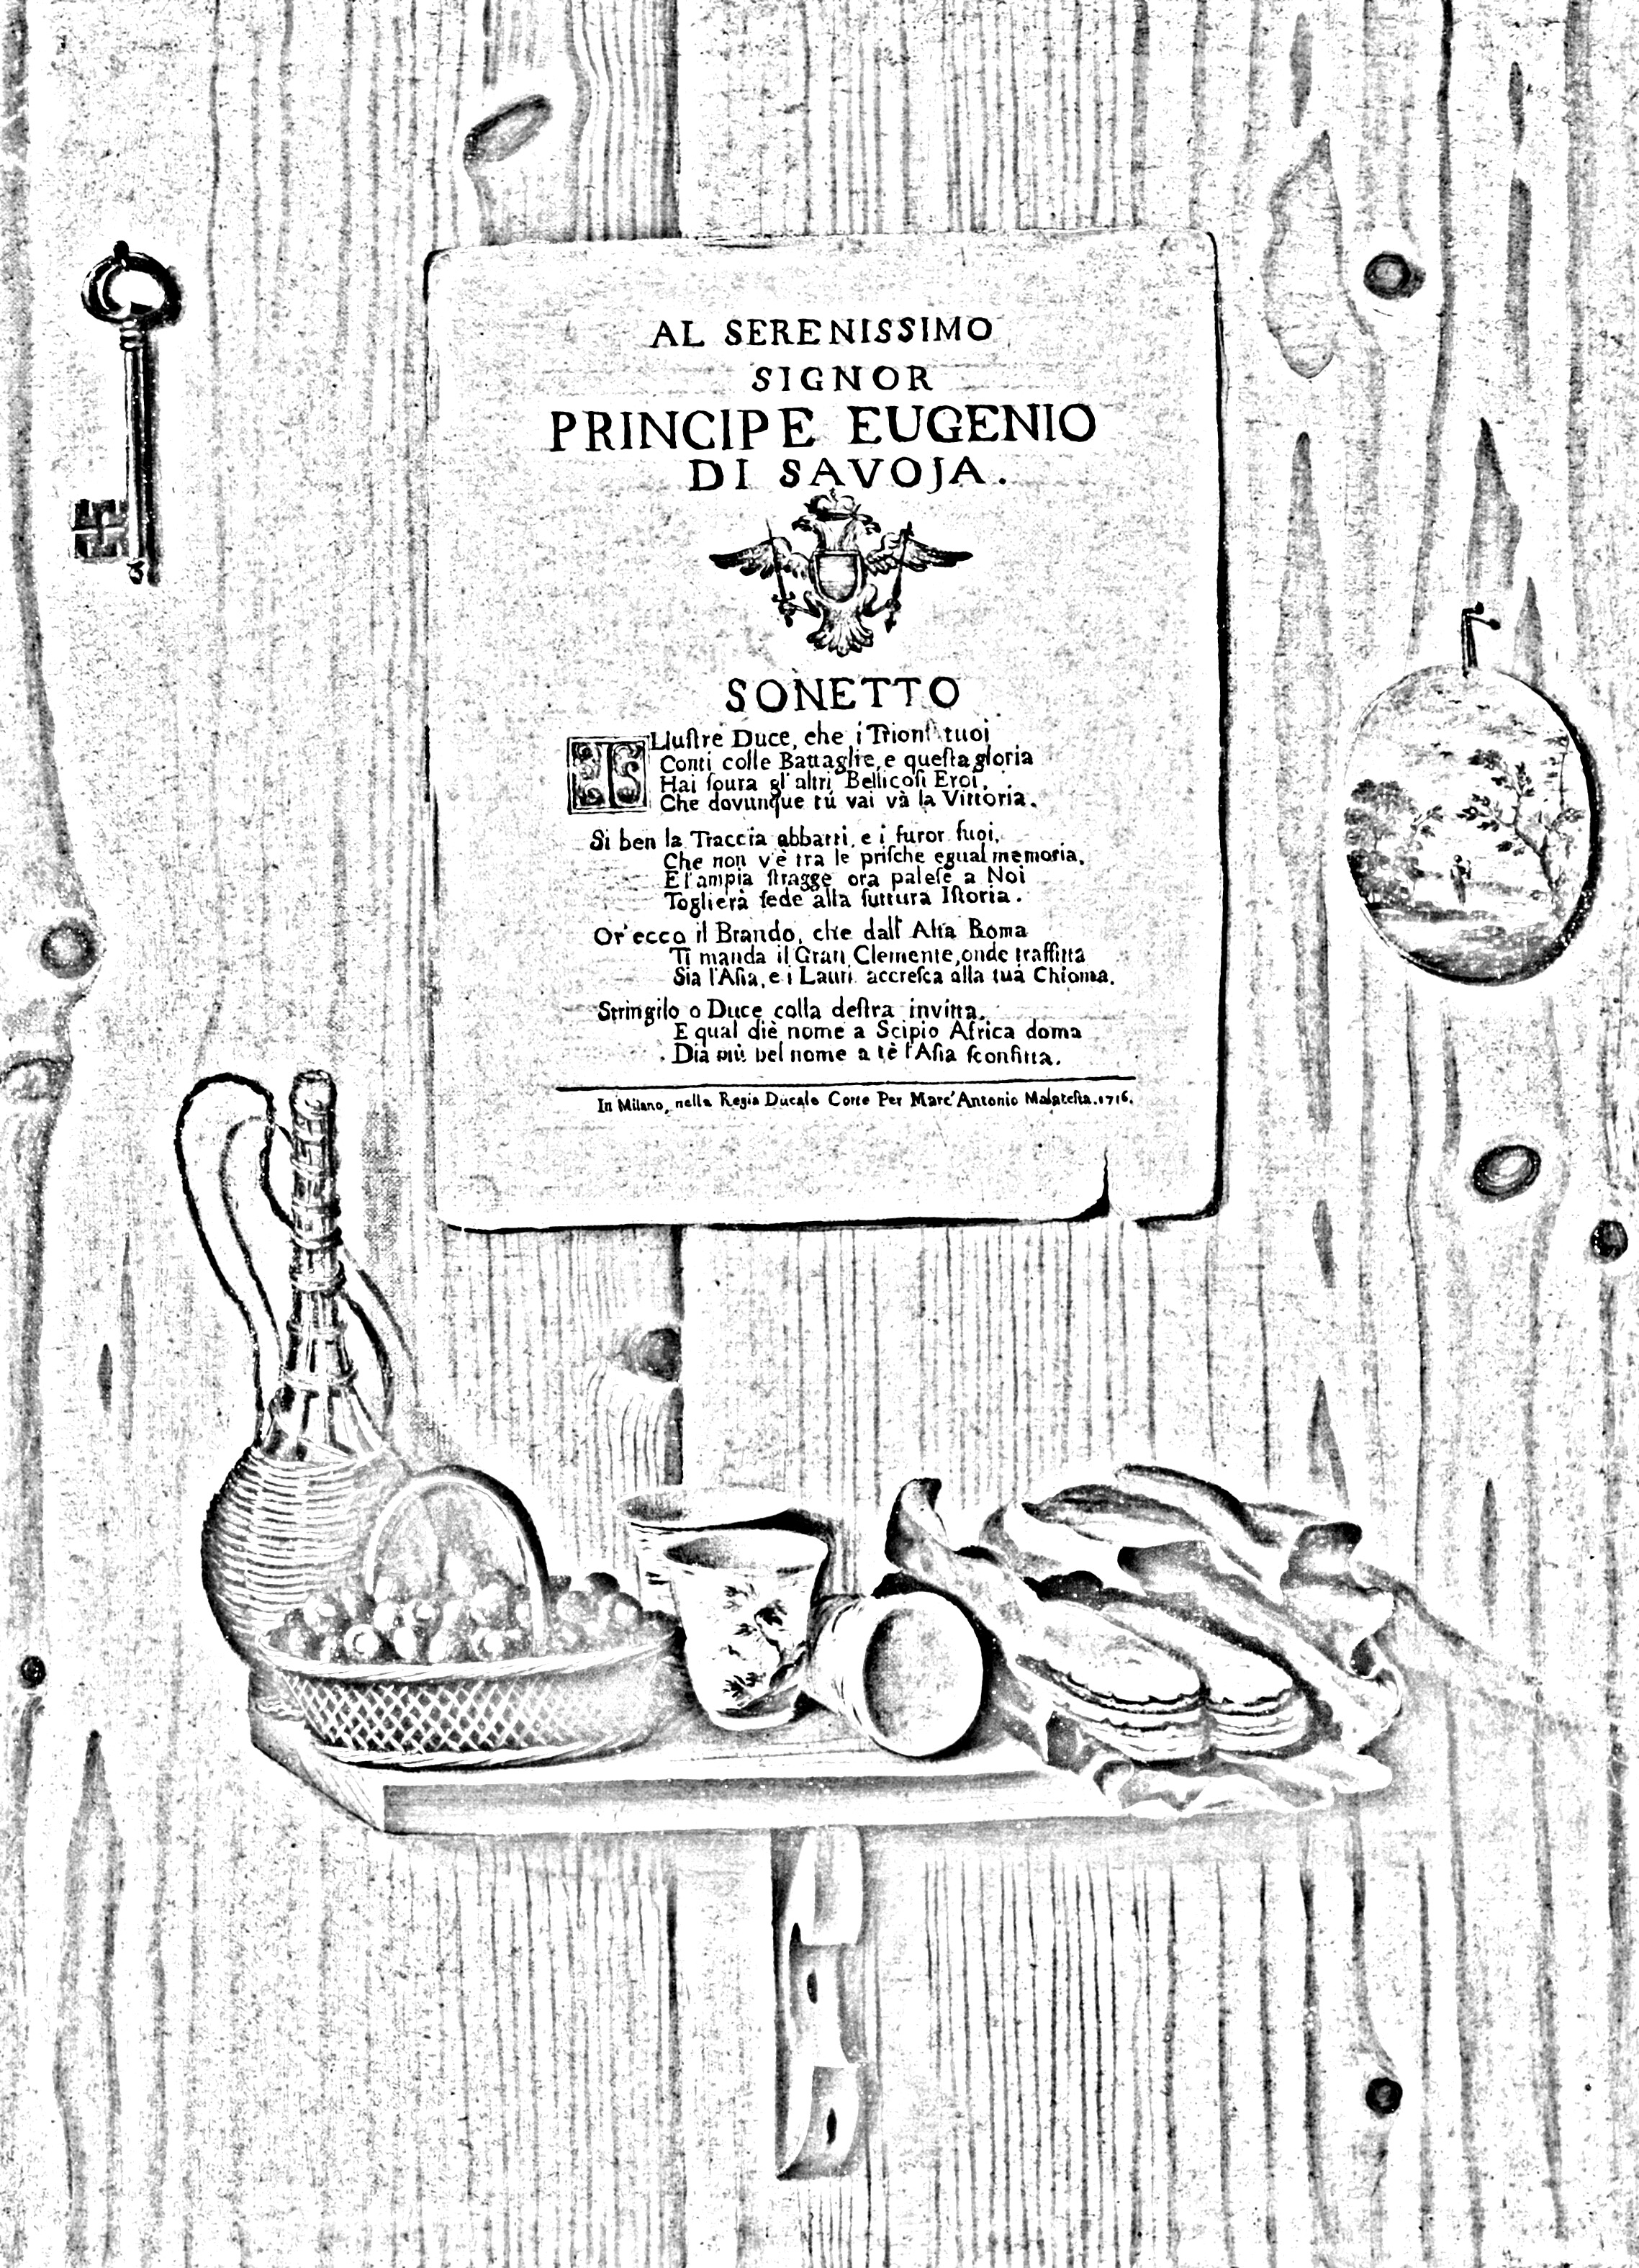
\includegraphics[scale=0.2]{Gianlisi_Antonio_Junior-Trompe_l_oeil_con_sonetto_in_onore_di_Eugenio_di_Savoia_e_mensola_con_oggetti.jpg}
			\end{minipage}
			
			\vspace*{\fill}
			\fboxrule=4pt{
				\fbox
				{
					\begin{minipage}[t][55pt][t]{0.91\linewidth}
						Gianlisi Antonio Junior - Trompe l'oeil con sonetto in onore di Eugenio di Savoia e mensola con oggetti - Colorato~da: 
					\end{minipage}
				}
			}
			\newpage
			
			%---------- Image ----------
			\thispagestyle{empty}
			\begin{minipage}{0.93\linewidth}
				\centering
				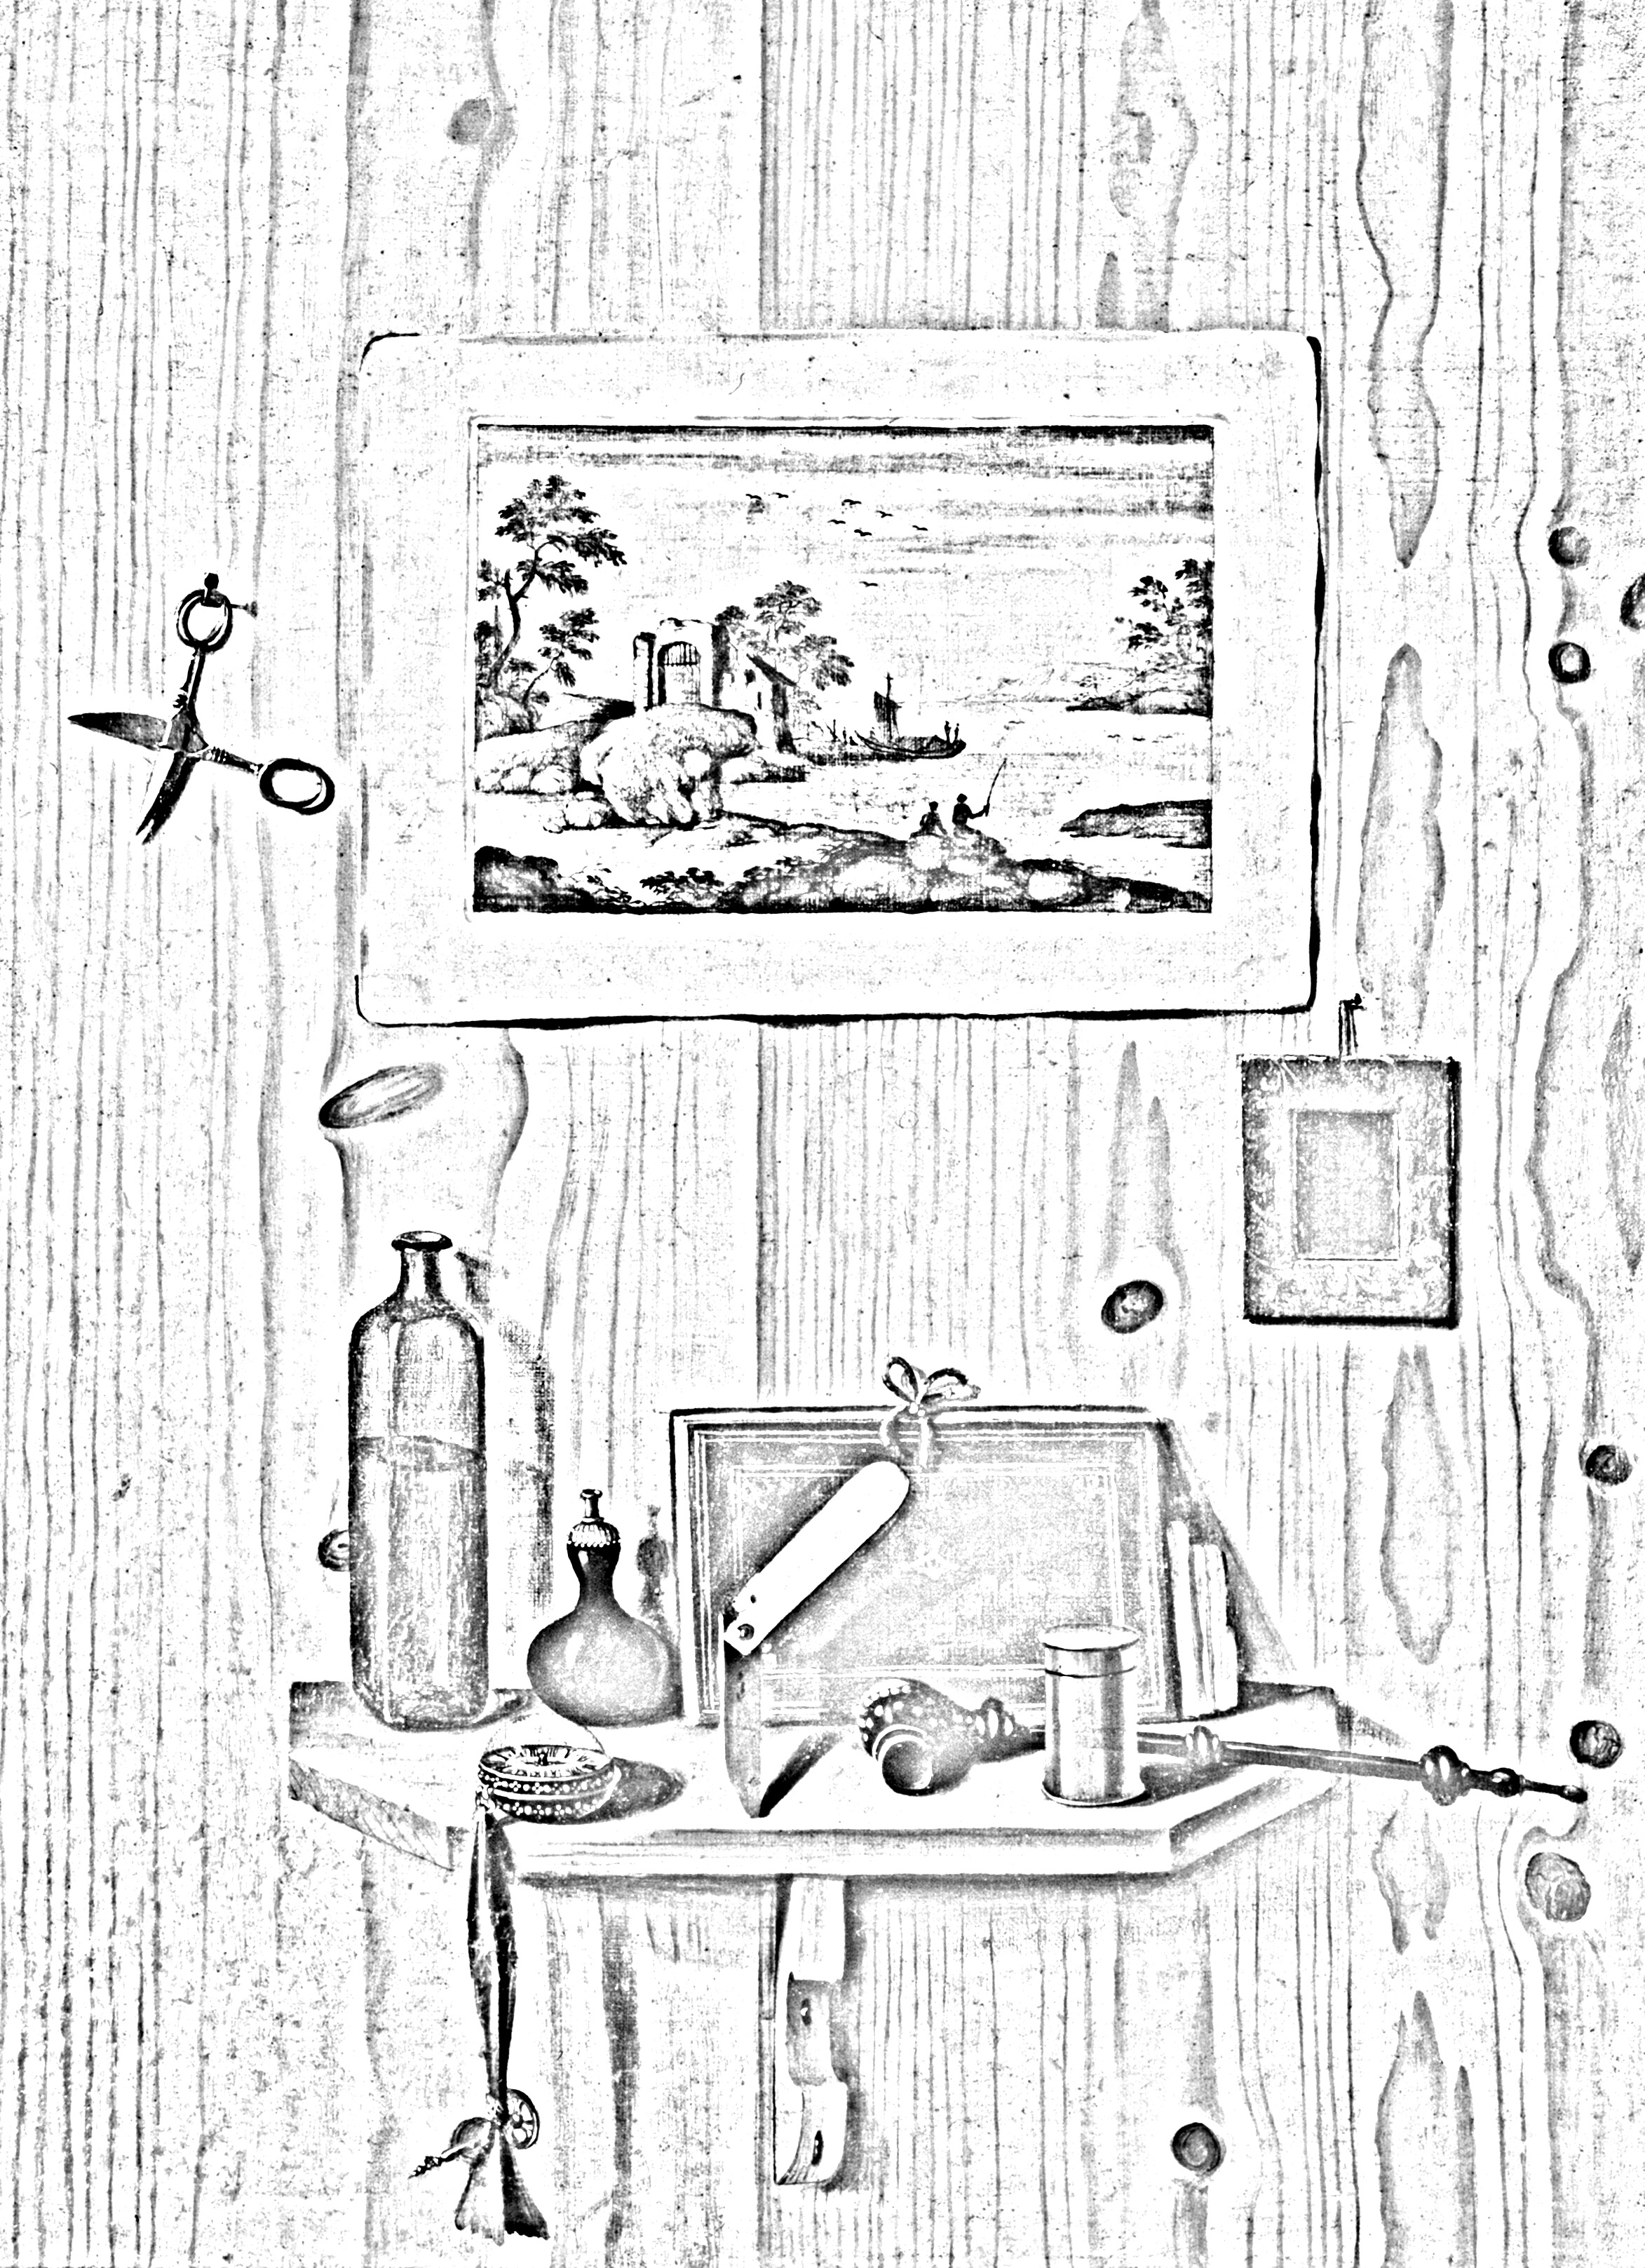
\includegraphics[scale=0.2]{Gianlisi_Antonio_Junior-Trompe_l_oeil_con_paesaggio_forbici_e_mensola_con_oggetti.jpg}
			\end{minipage}
			
			\vspace*{\fill}
			\fboxrule=4pt{
				\fbox
				{
					\begin{minipage}[t][55pt][t]{0.91\linewidth}
						Gianlisi Antonio Junior - Trompe l'oeil con paesaggio forbici e mensola con oggetti - \\Colorato~da: 
					\end{minipage}
				}
			}
			\newpage
			
			%---------- Image ----------
			\thispagestyle{empty}
			\begin{minipage}{0.94\linewidth}
				\centering
				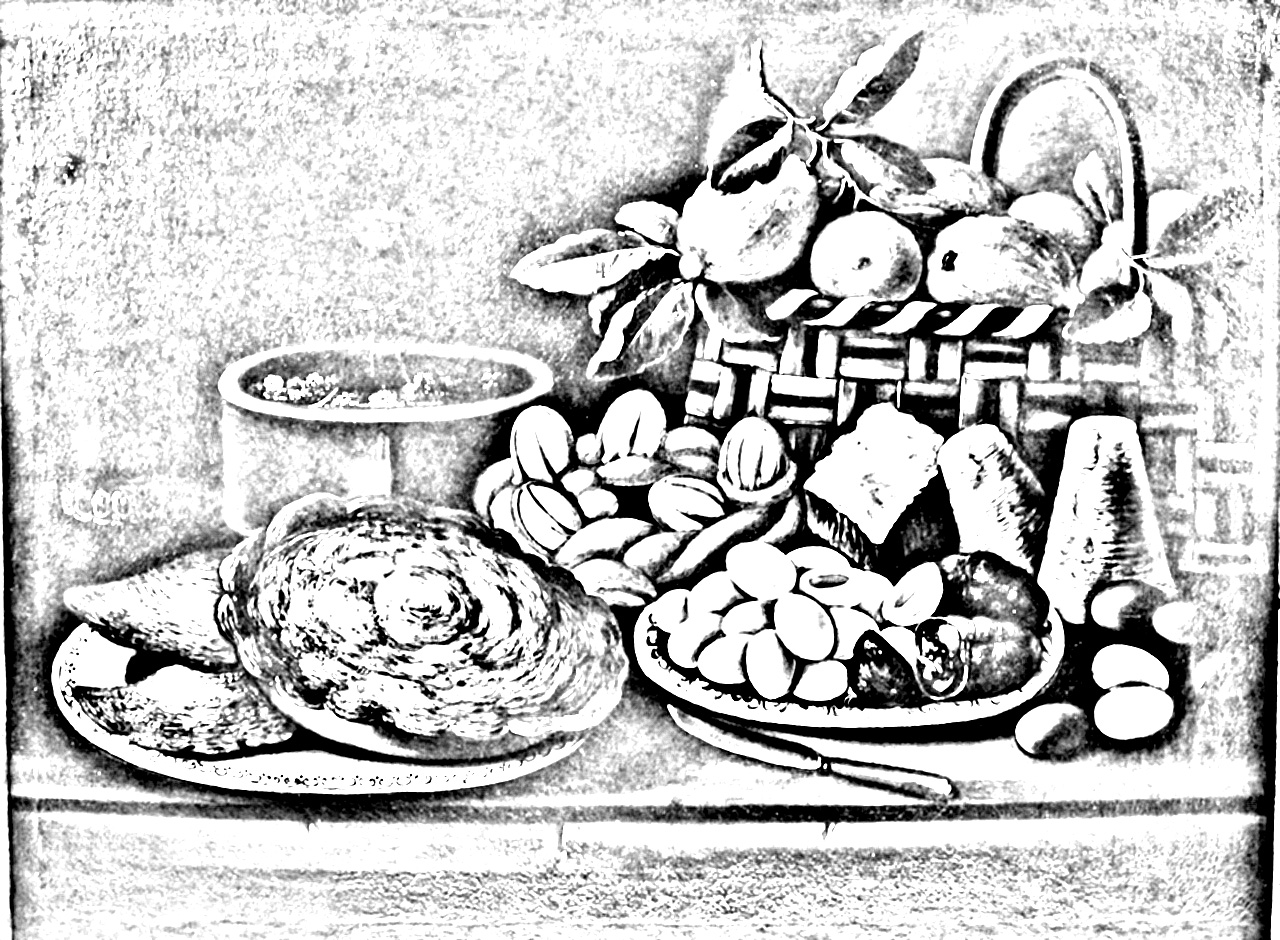
\includegraphics[scale=1.7]{Realfonzo_Tommaso-Natura_morta_con_dolci_frutta_uova_e_formaggi.jpg}
			\end{minipage}
			
			\vspace*{\fill}
			\fboxrule=4pt{
				\fbox
				{
					\begin{minipage}[t][55pt][t]{0.91\linewidth}
						Realfonzo Tommaso - Natura morta con dolci frutta uova e formaggi - Colorata da: 
					\end{minipage}
				}
			}
			\newpage
			
			%---------- Image ----------
			\thispagestyle{empty}
			\begin{minipage}{0.94\linewidth}
				\centering
				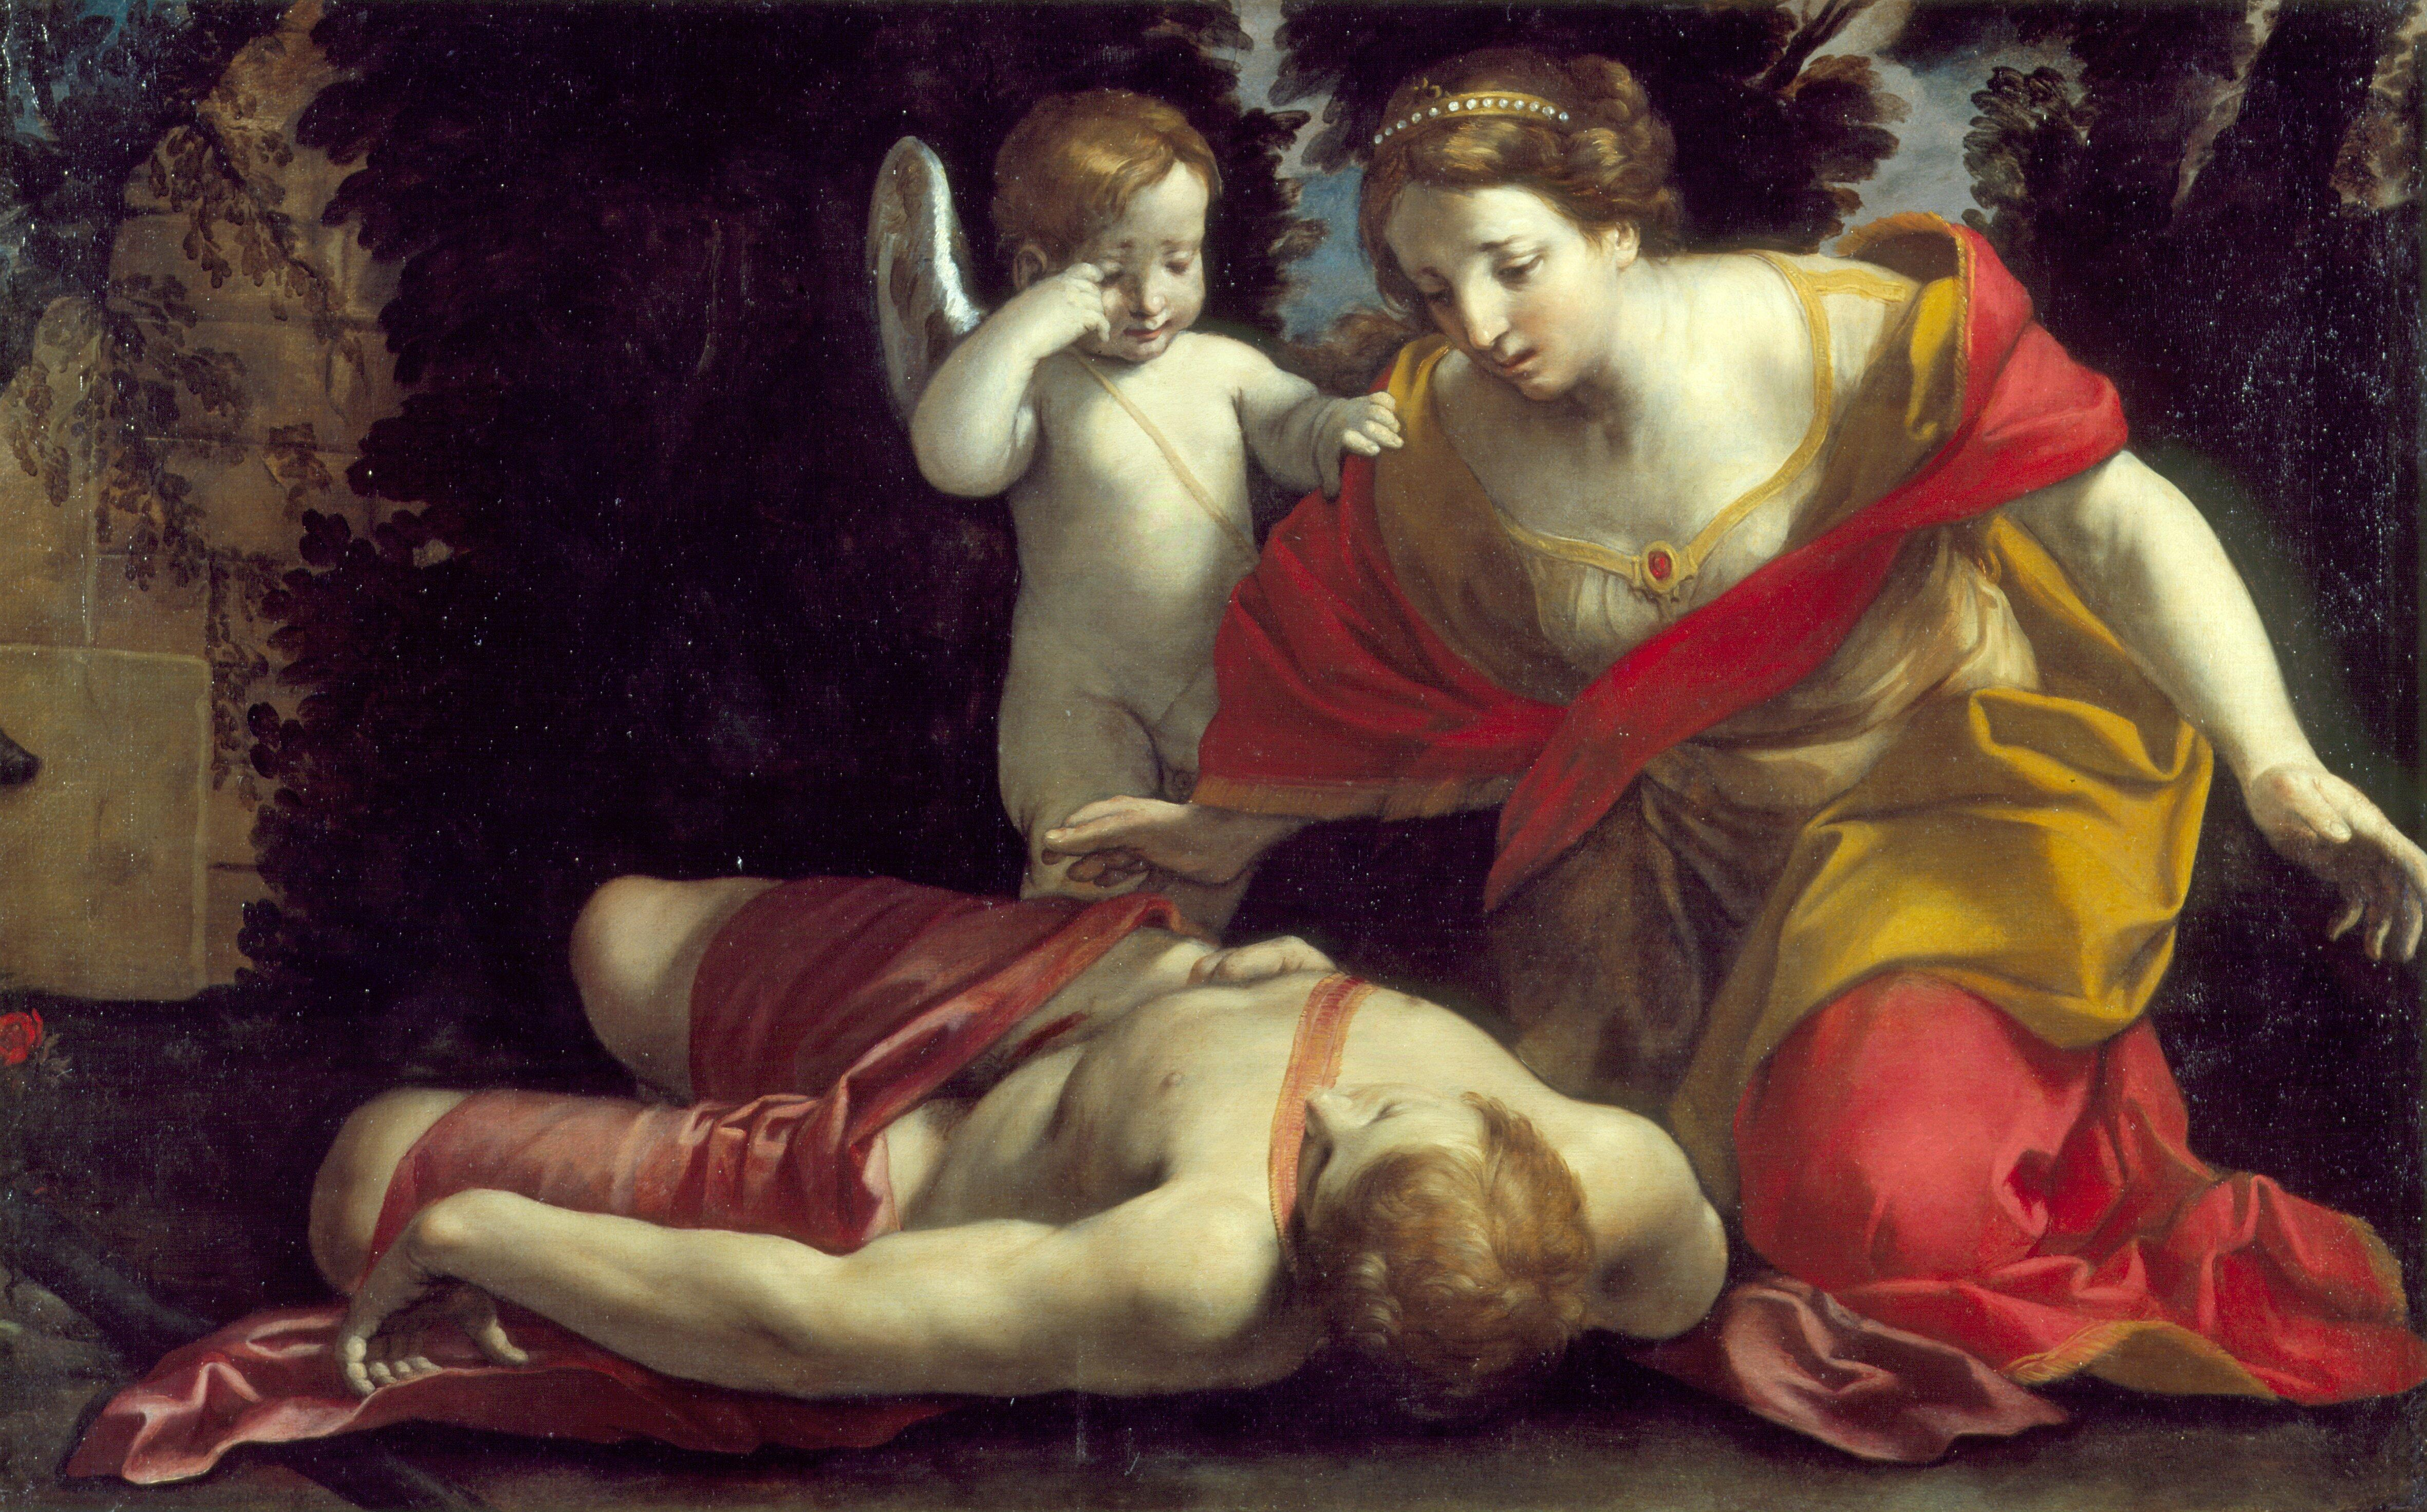
\includegraphics[scale=0.11]{Gessi_Giovan_Francesco-Morte_di_Adone.jpg}
			\end{minipage}
			
			\vspace*{\fill}
			\fboxrule=4pt{
				\fbox
				{
					\begin{minipage}[t][55pt][t]{0.91\linewidth}
					Gessi Giovan Francesco - Morte di Adone - Colorata da: 
					\end{minipage}
				}
			}
			\newpage
			
			\vspace*{\fill}
			% Print license shield
			\doclicenseThis
			
		\end{adjustwidth}
\end{document}